\documentclass[twoside]{article}

% Packages required by doxygen
\usepackage{fixltx2e}
\usepackage{calc}
\usepackage{doxygen}
\usepackage[export]{adjustbox} % also loads graphicx
\usepackage{graphicx}
\usepackage[utf8]{inputenc}
\usepackage{makeidx}
\usepackage{multicol}
\usepackage{multirow}
\PassOptionsToPackage{warn}{textcomp}
\usepackage{textcomp}
\usepackage[nointegrals]{wasysym}
\usepackage[table]{xcolor}

% NLS support packages
\usepackage[T2A]{fontenc}
\usepackage[russian]{babel}

% Font selection
\usepackage[T1]{fontenc}
\usepackage[scaled=.90]{helvet}
\usepackage{courier}
\usepackage{amssymb}
\usepackage{sectsty}
\renewcommand{\familydefault}{\sfdefault}
\allsectionsfont{%
  \fontseries{bc}\selectfont%
  \color{darkgray}%
}
\renewcommand{\DoxyLabelFont}{%
  \fontseries{bc}\selectfont%
  \color{darkgray}%
}
\newcommand{\+}{\discretionary{\mbox{\scriptsize$\hookleftarrow$}}{}{}}

% Page & text layout
\usepackage{geometry}
\geometry{%
  a4paper,%
  top=2.5cm,%
  bottom=2.5cm,%
  left=2.5cm,%
  right=2.5cm%
}
\tolerance=750
\hfuzz=15pt
\hbadness=750
\setlength{\emergencystretch}{15pt}
\setlength{\parindent}{0cm}
\setlength{\parskip}{0.2cm}
\makeatletter
\renewcommand{\paragraph}{%
  \@startsection{paragraph}{4}{0ex}{-1.0ex}{1.0ex}{%
    \normalfont\normalsize\bfseries\SS@parafont%
  }%
}
\renewcommand{\subparagraph}{%
  \@startsection{subparagraph}{5}{0ex}{-1.0ex}{1.0ex}{%
    \normalfont\normalsize\bfseries\SS@subparafont%
  }%
}
\makeatother

% Headers & footers
\usepackage{fancyhdr}
\pagestyle{fancyplain}
\fancyhead[LE]{\fancyplain{}{\bfseries\thepage}}
\fancyhead[CE]{\fancyplain{}{}}
\fancyhead[RE]{\fancyplain{}{\bfseries\leftmark}}
\fancyhead[LO]{\fancyplain{}{\bfseries\rightmark}}
\fancyhead[CO]{\fancyplain{}{}}
\fancyhead[RO]{\fancyplain{}{\bfseries\thepage}}
\fancyfoot[LE]{\fancyplain{}{}}
\fancyfoot[CE]{\fancyplain{}{}}
\fancyfoot[RE]{\fancyplain{}{\bfseries\scriptsize Документация по КДЗ модуль 3. }}
\fancyfoot[LO]{\fancyplain{}{\bfseries\scriptsize Документация по КДЗ модуль 3. }}
\fancyfoot[CO]{\fancyplain{}{}}
\fancyfoot[RO]{\fancyplain{}{}}
\renewcommand{\footrulewidth}{0.4pt}
\renewcommand{\sectionmark}[1]{%
  \markright{\thesection\ #1}%
}

% Indices & bibliography
\usepackage{natbib}
\usepackage[titles]{tocloft}
\setcounter{tocdepth}{3}
\setcounter{secnumdepth}{5}
\makeindex

% Custom commands
\newcommand{\clearemptydoublepage}{%
  \newpage{\pagestyle{empty}\cleardoublepage}%
}

% Custom packages
\usepackage{pdfpages}


%===== C O N T E N T S =====

\begin{document}

% Titlepage & ToC
\pagenumbering{roman}
\begin{titlepage}
\begin{center}
\vspace*{1cm}
{\large НАЦИОНАЛЬНЫЙ ИССЛЕДОВАТЕЛЬСКИЙ УНИВЕРСИТЕТ \\
«ВЫСШАЯ ШКОЛА ЭКОНОМИКИ» }\\
\vspace*{0.5cm}
{\large Факультет компьютерных наук }\\
\vspace*{0.5cm}
{\small Департамент программнoй инженерии \\
}
\vfill % заполняет длину страницы вертикально
{\large\textbf{
Контрольное домашнее задание \\
по дисциплине\\
«Программирование» \\
}}
\bigskip
{\large Тема работы: Обработка данных из файла }\\
\vfill
\begin{flushright}
Выполнил студент группы БПИ 151 \\
Абрамов А.M. \\
Преподаватель: Подбельский Вадим Валериевич \\
\end{flushright}
\vfill
Москва \number\year \\
Модуль 3
\end{center}
\end{titlepage}

\tableofcontents
\pagenumbering{arabic}

% --- add my custom headers ---
\section{Условие задачи}

\begin{DoxyImageNoCaption}
  \mbox{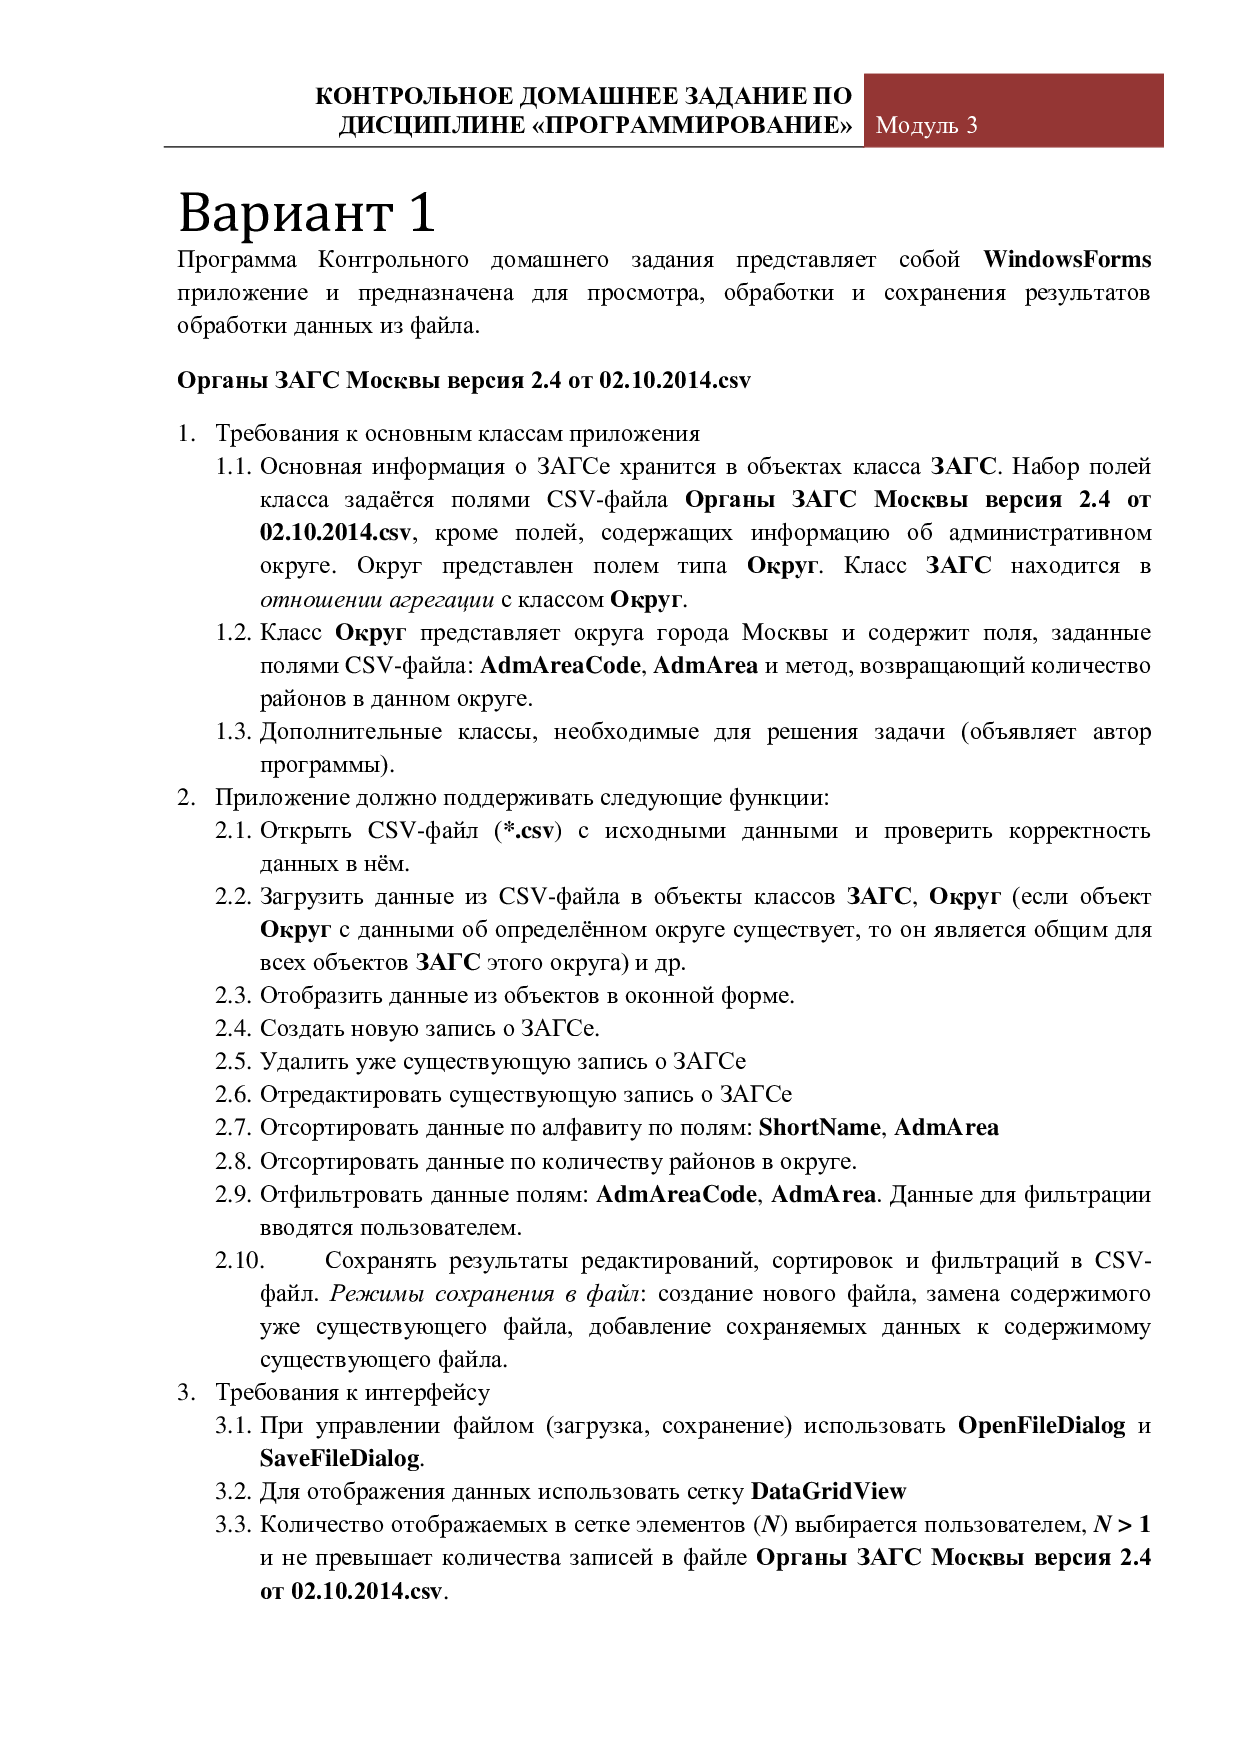
\includegraphics[height=22cm]{task_one.png}}
\end{DoxyImageNoCaption}
\newpage
\begin{DoxyImageNoCaption}
  \mbox{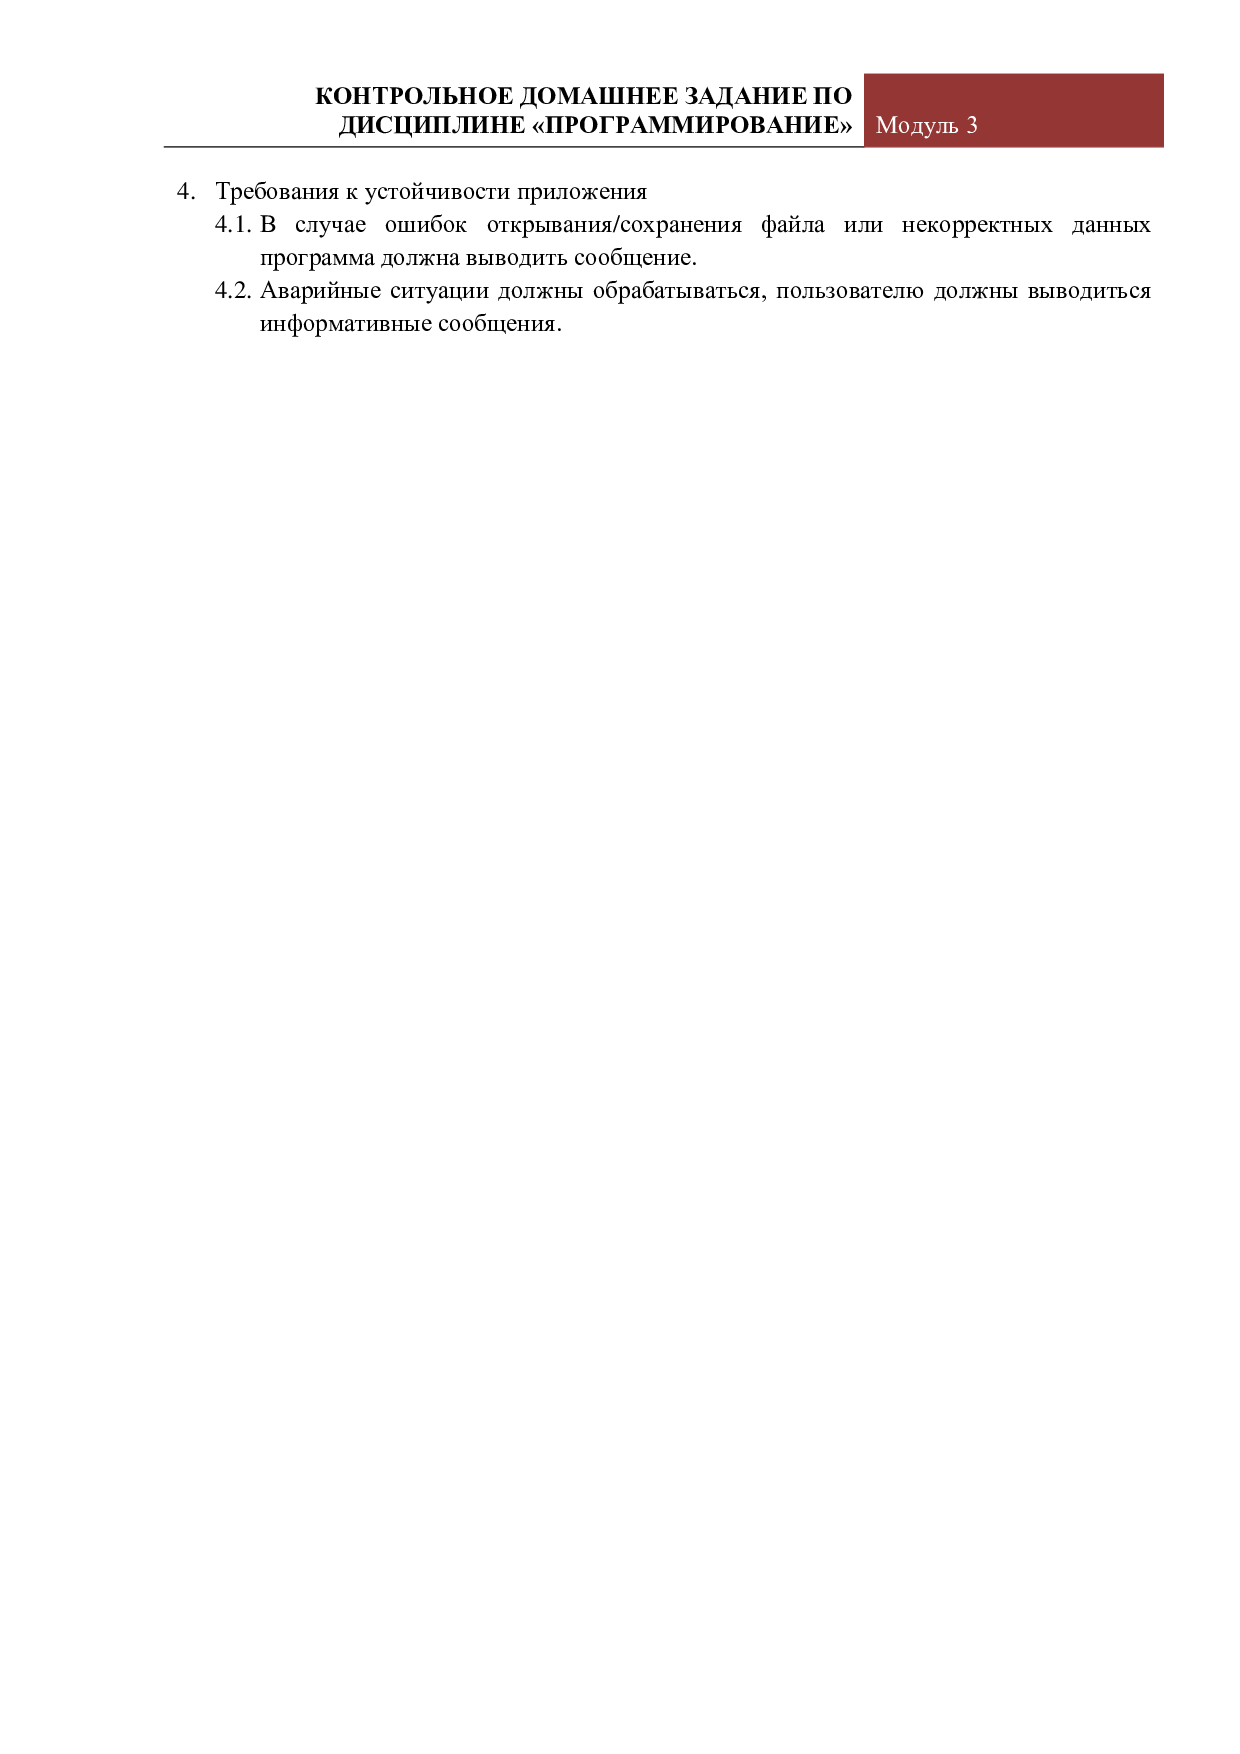
\includegraphics[height=22cm]{task_two.png}}
\end{DoxyImageNoCaption}
\newpage



\section{Функционал приложения}
\subsubsection*{Варианты использования}

Приложение позволяет просматривать C\+S\+V файлы. Просмотр данных из C\+S\+V файлов. Анализ частоты встречаемости данных. Поиск по базе данных записанной в формате C\+S\+V.

\subsubsection*{Описание интерфейса пользователя}

В программе присутствует стандартная верхняя панель меню и стандартная панель инструментов для работы с файлами. Для фильтрации данных в файле используются поля ввода расположенные над Data\+Grid\+View в котором отображаются данные из файла.

Для загрузки данных используется либо меню File, либо операцию Open на панели инструментов. Есть поддержка недавно открытых файлов. Также программа умеет запоминать последнюю посещенную директорию.

Сортировка колонок производится посредством щелканья на имени колонки. Фильтрация колонок производится посредством ввода значения для фильтра (то что должно совпадать). При поиске введенный регистр всегда учитывается. Также пользователь может воспользоваться продвинутым фильтром для более точной фильтрации.

Внизу программы представлен статус по данной таблице и по результатам фильтрации.

Также имеется поддержка для показа огранниченного набора строк и перелистывания страниц. Текущая страница и колличество строк на странице отображаются в вверху и слева от таблицы.

![alt text][interface\+\_\+menu] 
\section{Структура приложения}
![alt text][class\+\_\+diagram] 

%--- Begin generated contents ---
\section{Пространства имен}
\subsection{Пакет kdz\+\_\+manager}
\label{namespacekdz__manager}\index{kdz\+\_\+manager@{kdz\+\_\+manager}}
\subsubsection*{Пространства имен}
\begin{DoxyCompactItemize}
\item 
package {\bf Properties}
\end{DoxyCompactItemize}
\subsubsection*{Классы}
\begin{DoxyCompactItemize}
\item 
class {\bf Admin\+Area\+Data\+Row}
\begin{DoxyCompactList}\small\item\em Aggregates a number of books under the author\textquotesingle{}s name. \end{DoxyCompactList}\item 
class {\bf C\+S\+V\+Reader}
\begin{DoxyCompactList}\small\item\em Class to actually parse lines in C\+S\+V file. \end{DoxyCompactList}\item 
class {\bf C\+S\+V\+Writer}
\begin{DoxyCompactList}\small\item\em Class to serialize C\+S\+V data from data table to file. \end{DoxyCompactList}\item 
class {\bf Editor\+Text\+Box}
\item 
class {\bf Edit\+Row\+Form}
\item 
interface {\bf I\+From\+Map\+Data\+Row}
\item 
class {\bf Main\+Form}
\item 
class {\bf Map\+Data\+Row}
\begin{DoxyCompactList}\small\item\em Maps one row in C\+S\+V file to properties. \end{DoxyCompactList}\item 
class {\bf Open\+Data}
\item 
class {\bf Program}
\item 
class {\bf Recent\+Files\+Folders}
\item 
class {\bf Registry\+Office\+Data\+Row}
\begin{DoxyCompactList}\small\item\em Represents some books. \end{DoxyCompactList}\item 
class {\bf Save\+Data}
\item 
class {\bf View\+Data}
\end{DoxyCompactItemize}

\section{Классы}
\subsection{Класс Admin\+Area\+Data\+Row}
\label{classkdz__manager_1_1_admin_area_data_row}\index{Admin\+Area\+Data\+Row@{Admin\+Area\+Data\+Row}}


агрегатов ряд книг под именем автора.  


Граф наследования\+:Admin\+Area\+Data\+Row\+:\begin{figure}[H]
\begin{center}
\leavevmode
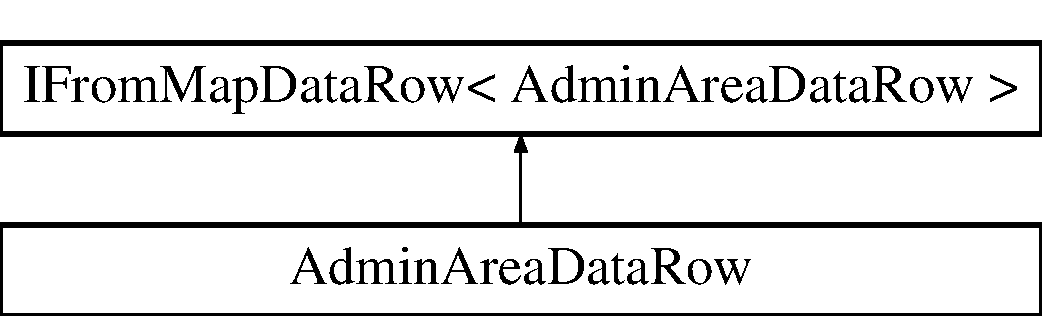
\includegraphics[height=2.000000cm]{classkdz__manager_1_1_admin_area_data_row}
\end{center}
\end{figure}
\subsubsection*{Открытые члены}
\begin{DoxyCompactItemize}
\item 
int {\bf Get\+Qty\+Of\+Distinct\+Book\+Prices} ()
\begin{DoxyCompactList}\small\item\em Возвращает количество различных цен на книги. (например, если три книги имеют ту же цену они считаться одним ) \end{DoxyCompactList}\item 
{\bf Admin\+Area\+Data\+Row} ()
\begin{DoxyCompactList}\small\item\em Беспараметрическая конструктор необходимо для использования в C\+S\+V парсер. \end{DoxyCompactList}\item 
{\bf Admin\+Area\+Data\+Row} ({\bf Map\+Data\+Row} input)
\begin{DoxyCompactList}\small\item\em Построить автора от карт Data\+Row \end{DoxyCompactList}\item 
{\bf Admin\+Area\+Data\+Row} {\bf From\+Map\+Data\+Row} ({\bf Map\+Data\+Row} input)
\begin{DoxyCompactList}\small\item\em Создать новый экземпляр из разобранного данных \end{DoxyCompactList}\end{DoxyCompactItemize}
\subsubsection*{Свойства}
\begin{DoxyCompactItemize}
\item 
string {\bfseries Adm\+Area}\hspace{0.3cm}{\ttfamily  [get, set]}\label{classkdz__manager_1_1_admin_area_data_row_a681cc5993f19cb1ddf82a5d7f139f724}

\item 
string {\bfseries Adm\+Area\+Code}\hspace{0.3cm}{\ttfamily  [get, set]}\label{classkdz__manager_1_1_admin_area_data_row_ab7eb47ebdd8dc4601e798df1860a76d4}

\item 
List$<$ {\bf Registry\+Office\+Data\+Row} $>$ {\bfseries Offices}\hspace{0.3cm}{\ttfamily  [get, set]}\label{classkdz__manager_1_1_admin_area_data_row_aba48dfff5f2b662e337093eb4fe4b702}

\end{DoxyCompactItemize}


\subsubsection{Подробное описание}


См. определение в файле Admin\+Area\+Data\+Row.\+cs строка 12



\subsubsection{Конструктор(ы)}
\index{kdz\+\_\+manager\+::\+Admin\+Area\+Data\+Row@{kdz\+\_\+manager\+::\+Admin\+Area\+Data\+Row}!Admin\+Area\+Data\+Row@{Admin\+Area\+Data\+Row}}
\index{Admin\+Area\+Data\+Row@{Admin\+Area\+Data\+Row}!kdz\+\_\+manager\+::\+Admin\+Area\+Data\+Row@{kdz\+\_\+manager\+::\+Admin\+Area\+Data\+Row}}
\paragraph[{Admin\+Area\+Data\+Row()}]{\setlength{\rightskip}{0pt plus 5cm}{\bf Admin\+Area\+Data\+Row} (
\begin{DoxyParamCaption}
{}
\end{DoxyParamCaption}
)}\label{classkdz__manager_1_1_admin_area_data_row_a5773cde8c1f167eef314d4e86063dac5_a5773cde8c1f167eef314d4e86063dac5}


См. определение в файле Admin\+Area\+Data\+Row.\+cs строка 31

\index{kdz\+\_\+manager\+::\+Admin\+Area\+Data\+Row@{kdz\+\_\+manager\+::\+Admin\+Area\+Data\+Row}!Admin\+Area\+Data\+Row@{Admin\+Area\+Data\+Row}}
\index{Admin\+Area\+Data\+Row@{Admin\+Area\+Data\+Row}!kdz\+\_\+manager\+::\+Admin\+Area\+Data\+Row@{kdz\+\_\+manager\+::\+Admin\+Area\+Data\+Row}}
\paragraph[{Admin\+Area\+Data\+Row(\+Map\+Data\+Row input)}]{\setlength{\rightskip}{0pt plus 5cm}{\bf Admin\+Area\+Data\+Row} (
\begin{DoxyParamCaption}
\item[{{\bf Map\+Data\+Row}}]{input}
\end{DoxyParamCaption}
)}\label{classkdz__manager_1_1_admin_area_data_row_a558afd5a9f13d31405d60a7aecf6aeef_a558afd5a9f13d31405d60a7aecf6aeef}

\begin{DoxyParams}{Аргументы}
{\em input} & \\
\hline
\end{DoxyParams}


См. определение в файле Admin\+Area\+Data\+Row.\+cs строка 42



\subsubsection{Методы}
\index{kdz\+\_\+manager\+::\+Admin\+Area\+Data\+Row@{kdz\+\_\+manager\+::\+Admin\+Area\+Data\+Row}!From\+Map\+Data\+Row@{From\+Map\+Data\+Row}}
\index{From\+Map\+Data\+Row@{From\+Map\+Data\+Row}!kdz\+\_\+manager\+::\+Admin\+Area\+Data\+Row@{kdz\+\_\+manager\+::\+Admin\+Area\+Data\+Row}}
\paragraph[{From\+Map\+Data\+Row(\+Map\+Data\+Row input)}]{\setlength{\rightskip}{0pt plus 5cm}{\bf Admin\+Area\+Data\+Row} From\+Map\+Data\+Row (
\begin{DoxyParamCaption}
\item[{{\bf Map\+Data\+Row}}]{input}
\end{DoxyParamCaption}
)}\label{classkdz__manager_1_1_admin_area_data_row_a01eb541f272c3ddc0d435fd1ce1b4537_a01eb541f272c3ddc0d435fd1ce1b4537}
\begin{DoxyReturn}{Возвращает}

\end{DoxyReturn}


См. определение в файле Admin\+Area\+Data\+Row.\+cs строка 53

\index{kdz\+\_\+manager\+::\+Admin\+Area\+Data\+Row@{kdz\+\_\+manager\+::\+Admin\+Area\+Data\+Row}!Get\+Qty\+Of\+Distinct\+Book\+Prices@{Get\+Qty\+Of\+Distinct\+Book\+Prices}}
\index{Get\+Qty\+Of\+Distinct\+Book\+Prices@{Get\+Qty\+Of\+Distinct\+Book\+Prices}!kdz\+\_\+manager\+::\+Admin\+Area\+Data\+Row@{kdz\+\_\+manager\+::\+Admin\+Area\+Data\+Row}}
\paragraph[{Get\+Qty\+Of\+Distinct\+Book\+Prices()}]{\setlength{\rightskip}{0pt plus 5cm}int Get\+Qty\+Of\+Distinct\+Book\+Prices (
\begin{DoxyParamCaption}
{}
\end{DoxyParamCaption}
)}\label{classkdz__manager_1_1_admin_area_data_row_ad29cc131822e3f36b0e61ff3a9bbac47_ad29cc131822e3f36b0e61ff3a9bbac47}
\begin{DoxyReturn}{Возвращает}

\end{DoxyReturn}


См. определение в файле Admin\+Area\+Data\+Row.\+cs строка 23


\subsection{Класс C\+S\+V\+Reader}
\label{classkdz__manager_1_1_c_s_v_reader}\index{C\+S\+V\+Reader@{C\+S\+V\+Reader}}


Класс фактически разобрать строки в C\+S\+V -\/файл.  


Граф наследования\+:C\+S\+V\+Reader\+:\begin{figure}[H]
\begin{center}
\leavevmode
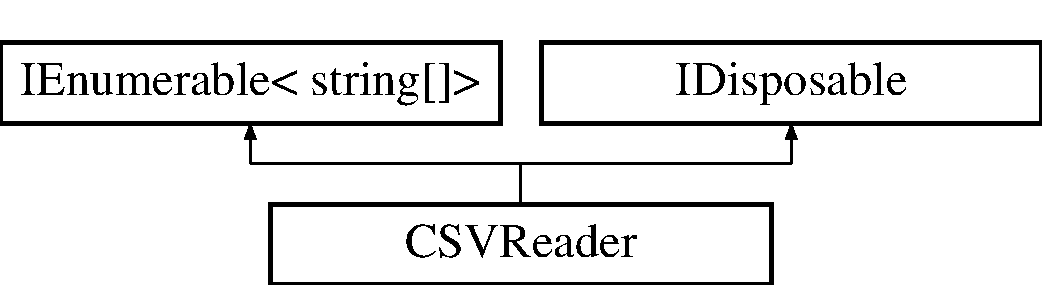
\includegraphics[height=2.000000cm]{classkdz__manager_1_1_c_s_v_reader}
\end{center}
\end{figure}
\subsubsection*{Открытые члены}
\begin{DoxyCompactItemize}
\item 
{\bf C\+S\+V\+Reader} (Stream\+Reader source, char separator, char text\+\_\+escape)
\begin{DoxyCompactList}\small\item\em Построить новый читатель C\+S\+V от источника потока \end{DoxyCompactList}\item 
I\+Enumerable$<$ string[$\,$]$>$ {\bf Get\+Lines} ()
\begin{DoxyCompactList}\small\item\em перебора всех строк этого файла C\+S\+V \end{DoxyCompactList}\item 
string[$\,$] {\bf Next\+Line} ()
\begin{DoxyCompactList}\small\item\em Получить следующую строку из файла. \end{DoxyCompactList}\item 
void {\bf Dispose} ()
\begin{DoxyCompactList}\small\item\em закрывать ресурсы -\/ в частности, читатель поток \end{DoxyCompactList}\item 
List$<$ T $>$ {\bf Deserialize$<$ T $>$} ()
\begin{DoxyCompactList}\small\item\em десериализации C\+S\+V файл в списке набранных объектов \end{DoxyCompactList}\item 
string[$\,$] {\bf Parse\+Multi\+Line} (Stream\+Reader sr)
\begin{DoxyCompactList}\small\item\em Разбор линию, значения которого могут включать новые символы строки или C\+R / L\+F \end{DoxyCompactList}\item 
string[$\,$] {\bf Parse\+Line} (string s)
\begin{DoxyCompactList}\small\item\em Разбор строки и вернуть массив, если это удастся, или в лучшем случае как мы можем получить \end{DoxyCompactList}\item 
bool {\bf Try\+Parse\+Line} (string s, out string[$\,$] array)
\begin{DoxyCompactList}\small\item\em прочитал в строке текста, а также использовать функцию Add (), чтобы добавить эти элементы к существующей структуре C\+S\+V \end{DoxyCompactList}\end{DoxyCompactItemize}


\subsubsection{Подробное описание}


См. определение в файле Open\+Data.\+cs строка 17



\subsubsection{Конструктор(ы)}
\index{kdz\+\_\+manager\+::\+C\+S\+V\+Reader@{kdz\+\_\+manager\+::\+C\+S\+V\+Reader}!C\+S\+V\+Reader@{C\+S\+V\+Reader}}
\index{C\+S\+V\+Reader@{C\+S\+V\+Reader}!kdz\+\_\+manager\+::\+C\+S\+V\+Reader@{kdz\+\_\+manager\+::\+C\+S\+V\+Reader}}
\paragraph[{C\+S\+V\+Reader(\+Stream\+Reader source, char separator, char text\+\_\+escape)}]{\setlength{\rightskip}{0pt plus 5cm}{\bf C\+S\+V\+Reader} (
\begin{DoxyParamCaption}
\item[{Stream\+Reader}]{source, }
\item[{char}]{separator, }
\item[{char}]{text\+\_\+escape}
\end{DoxyParamCaption}
)}\label{classkdz__manager_1_1_c_s_v_reader_ac368737bf9ddbb9cb351f00c3cacda20_ac368737bf9ddbb9cb351f00c3cacda20}

\begin{DoxyParams}{Аргументы}
{\em source} & \\
\hline
{\em separator} & \\
\hline
{\em text\+\_\+escape} & \\
\hline
\end{DoxyParams}


См. определение в файле Open\+Data.\+cs строка 32



\subsubsection{Методы}
\index{kdz\+\_\+manager\+::\+C\+S\+V\+Reader@{kdz\+\_\+manager\+::\+C\+S\+V\+Reader}!Deserialize$<$ T $>$@{Deserialize$<$ T $>$}}
\index{Deserialize$<$ T $>$@{Deserialize$<$ T $>$}!kdz\+\_\+manager\+::\+C\+S\+V\+Reader@{kdz\+\_\+manager\+::\+C\+S\+V\+Reader}}
\paragraph[{Deserialize$<$ T $>$()}]{\setlength{\rightskip}{0pt plus 5cm}List$<$T$>$ Deserialize$<$ T $>$ (
\begin{DoxyParamCaption}
{}
\end{DoxyParamCaption}
)}\label{classkdz__manager_1_1_c_s_v_reader_ab826689c78796b51d5cd7b169ebf98b6_ab826689c78796b51d5cd7b169ebf98b6}

\begin{DoxyTemplParams}{Template Parameters}
{\em T} & The type of objects to deserialize from this C\+S\+V.\\
\hline
\end{DoxyTemplParams}
\begin{DoxyReturn}{Возвращает}
An array of objects that were retrieved from the C\+S\+V file.
\end{DoxyReturn}
\begin{Desc}
\item[Согласование типов]\begin{description}
\item[{\em T} : {\em class}]\item[{\em T} : {\em new()}]\end{description}
\end{Desc}


См. определение в файле Open\+Data.\+cs строка 100

\index{kdz\+\_\+manager\+::\+C\+S\+V\+Reader@{kdz\+\_\+manager\+::\+C\+S\+V\+Reader}!Dispose@{Dispose}}
\index{Dispose@{Dispose}!kdz\+\_\+manager\+::\+C\+S\+V\+Reader@{kdz\+\_\+manager\+::\+C\+S\+V\+Reader}}
\paragraph[{Dispose()}]{\setlength{\rightskip}{0pt plus 5cm}void Dispose (
\begin{DoxyParamCaption}
{}
\end{DoxyParamCaption}
)}\label{classkdz__manager_1_1_c_s_v_reader_a6e2d745cdb7a7b983f861ed6a9a541a7_a6e2d745cdb7a7b983f861ed6a9a541a7}


См. определение в файле Open\+Data.\+cs строка 89

\index{kdz\+\_\+manager\+::\+C\+S\+V\+Reader@{kdz\+\_\+manager\+::\+C\+S\+V\+Reader}!Get\+Lines@{Get\+Lines}}
\index{Get\+Lines@{Get\+Lines}!kdz\+\_\+manager\+::\+C\+S\+V\+Reader@{kdz\+\_\+manager\+::\+C\+S\+V\+Reader}}
\paragraph[{Get\+Lines()}]{\setlength{\rightskip}{0pt plus 5cm}I\+Enumerable$<$string[$\,$]$>$ Get\+Lines (
\begin{DoxyParamCaption}
{}
\end{DoxyParamCaption}
)}\label{classkdz__manager_1_1_c_s_v_reader_ae72278a935106bdf1717fea8d2a6bda4_ae72278a935106bdf1717fea8d2a6bda4}
\begin{DoxyReturn}{Возвращает}
An array of all data columns in the line
\end{DoxyReturn}


См. определение в файле Open\+Data.\+cs строка 61

\index{kdz\+\_\+manager\+::\+C\+S\+V\+Reader@{kdz\+\_\+manager\+::\+C\+S\+V\+Reader}!Next\+Line@{Next\+Line}}
\index{Next\+Line@{Next\+Line}!kdz\+\_\+manager\+::\+C\+S\+V\+Reader@{kdz\+\_\+manager\+::\+C\+S\+V\+Reader}}
\paragraph[{Next\+Line()}]{\setlength{\rightskip}{0pt plus 5cm}string [$\,$] Next\+Line (
\begin{DoxyParamCaption}
{}
\end{DoxyParamCaption}
)}\label{classkdz__manager_1_1_c_s_v_reader_aa2edaf8d7d8ab24d318b8fb54d7bc9d6_aa2edaf8d7d8ab24d318b8fb54d7bc9d6}
\begin{DoxyReturn}{Возвращает}
One line from the file.
\end{DoxyReturn}


См. определение в файле Open\+Data.\+cs строка 81

\index{kdz\+\_\+manager\+::\+C\+S\+V\+Reader@{kdz\+\_\+manager\+::\+C\+S\+V\+Reader}!Parse\+Line@{Parse\+Line}}
\index{Parse\+Line@{Parse\+Line}!kdz\+\_\+manager\+::\+C\+S\+V\+Reader@{kdz\+\_\+manager\+::\+C\+S\+V\+Reader}}
\paragraph[{Parse\+Line(string s)}]{\setlength{\rightskip}{0pt plus 5cm}string [$\,$] Parse\+Line (
\begin{DoxyParamCaption}
\item[{string}]{s}
\end{DoxyParamCaption}
)}\label{classkdz__manager_1_1_c_s_v_reader_ab017555795c09b898ff49d06bf6bc24a_ab017555795c09b898ff49d06bf6bc24a}

\begin{DoxyParams}{Аргументы}
{\em s} & \\
\hline
\end{DoxyParams}
\begin{DoxyReturn}{Возвращает}

\end{DoxyReturn}


См. определение в файле Open\+Data.\+cs строка 216

\index{kdz\+\_\+manager\+::\+C\+S\+V\+Reader@{kdz\+\_\+manager\+::\+C\+S\+V\+Reader}!Parse\+Multi\+Line@{Parse\+Multi\+Line}}
\index{Parse\+Multi\+Line@{Parse\+Multi\+Line}!kdz\+\_\+manager\+::\+C\+S\+V\+Reader@{kdz\+\_\+manager\+::\+C\+S\+V\+Reader}}
\paragraph[{Parse\+Multi\+Line(\+Stream\+Reader sr)}]{\setlength{\rightskip}{0pt plus 5cm}string [$\,$] Parse\+Multi\+Line (
\begin{DoxyParamCaption}
\item[{Stream\+Reader}]{sr}
\end{DoxyParamCaption}
)}\label{classkdz__manager_1_1_c_s_v_reader_a78c48cf76d5e5b05a7024caee6da2880_a78c48cf76d5e5b05a7024caee6da2880}

\begin{DoxyParams}{Аргументы}
{\em sr} & \\
\hline
\end{DoxyParams}
\begin{DoxyReturn}{Возвращает}

\end{DoxyReturn}


См. определение в файле Open\+Data.\+cs строка 186

\index{kdz\+\_\+manager\+::\+C\+S\+V\+Reader@{kdz\+\_\+manager\+::\+C\+S\+V\+Reader}!Try\+Parse\+Line@{Try\+Parse\+Line}}
\index{Try\+Parse\+Line@{Try\+Parse\+Line}!kdz\+\_\+manager\+::\+C\+S\+V\+Reader@{kdz\+\_\+manager\+::\+C\+S\+V\+Reader}}
\paragraph[{Try\+Parse\+Line(string s, out string[] array)}]{\setlength{\rightskip}{0pt plus 5cm}bool Try\+Parse\+Line (
\begin{DoxyParamCaption}
\item[{string}]{s, }
\item[{out string[$\,$]}]{array}
\end{DoxyParamCaption}
)}\label{classkdz__manager_1_1_c_s_v_reader_af8102a03b7b1aa448fea0f8cbd7eaaa8_af8102a03b7b1aa448fea0f8cbd7eaaa8}

\begin{DoxyParams}{Аргументы}
{\em s} & \\
\hline
\end{DoxyParams}


См. определение в файле Open\+Data.\+cs строка 227


\subsection{Класс C\+S\+V\+Writer}
\label{classkdz__manager_1_1_c_s_v_writer}\index{C\+S\+V\+Writer@{C\+S\+V\+Writer}}


Class to serialize C\+S\+V data from data table to file.  


Граф наследования\+:C\+S\+V\+Writer\+:\begin{figure}[H]
\begin{center}
\leavevmode
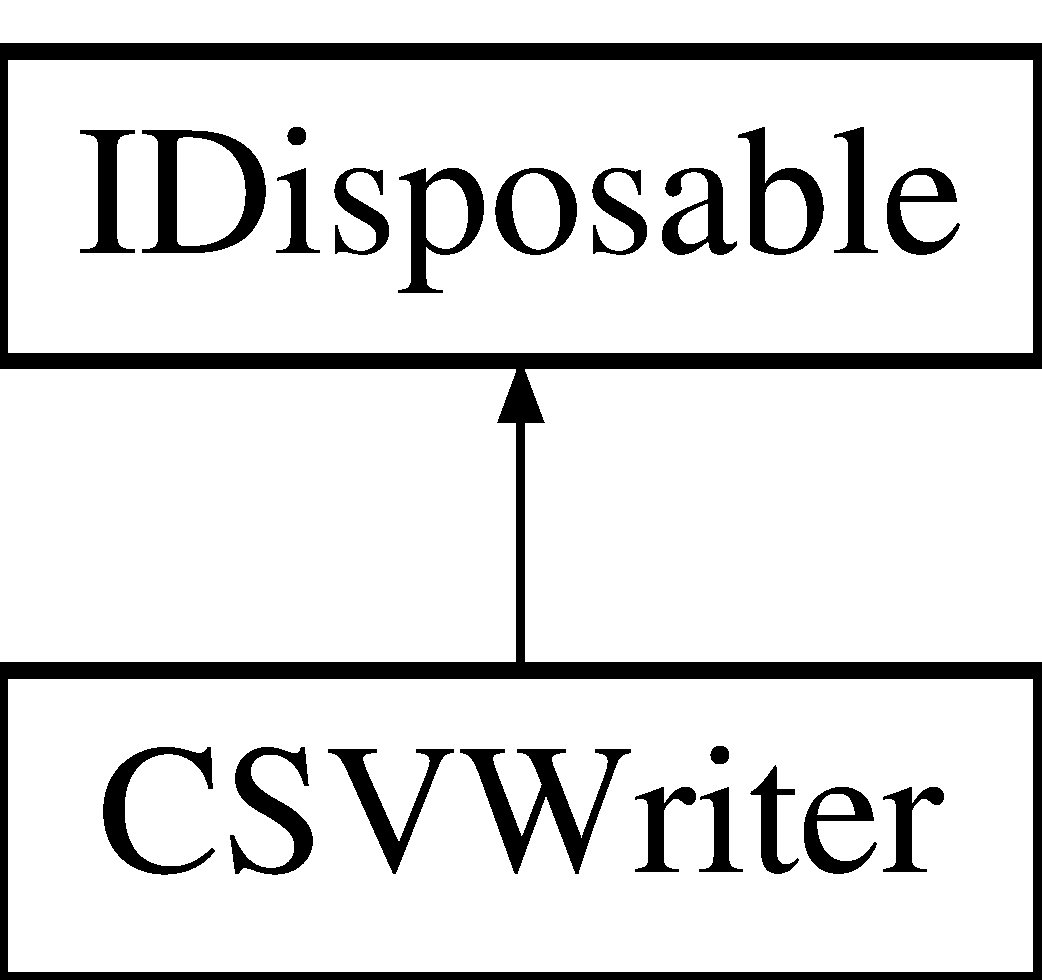
\includegraphics[height=2.000000cm]{classkdz__manager_1_1_c_s_v_writer}
\end{center}
\end{figure}
\subsubsection*{Открытые члены}
\begin{DoxyCompactItemize}
\item 
{\bf C\+S\+V\+Writer} (Stream\+Writer source, char separator, char text\+\_\+escape)
\begin{DoxyCompactList}\small\item\em Construct a new C\+S\+V writer to produce output on the enclosed Stream\+Writer \end{DoxyCompactList}\item 
void {\bf Write$<$ T $>$} (Data\+Table dt, bool write\+\_\+header)
\begin{DoxyCompactList}\small\item\em Write the data table to a stream in C\+S\+V format \end{DoxyCompactList}\item 
void {\bf Dispose} ()
\begin{DoxyCompactList}\small\item\em Close our resources -\/ specifically, the stream reader \end{DoxyCompactList}\item 
void {\bf Write\+Line} (I\+Enumerable$<$ object $>$ line)
\begin{DoxyCompactList}\small\item\em Write one line to the file \end{DoxyCompactList}\item 
string {\bf Make\+Output} (I\+Enumerable$<$ object $>$ line)
\begin{DoxyCompactList}\small\item\em Output a single field value as appropriate \end{DoxyCompactList}\end{DoxyCompactItemize}
\subsubsection*{Защищенные данные}
\begin{DoxyCompactItemize}
\item 
Stream\+Writer {\bfseries \+\_\+outstream}\label{classkdz__manager_1_1_c_s_v_writer_a0d60c35e43981c0780523edaf95392a5}

\end{DoxyCompactItemize}


\subsubsection{Подробное описание}


См. определение в файле Save\+Data.\+cs строка 17



\subsubsection{Конструктор(ы)}
\index{kdz\+\_\+manager\+::\+C\+S\+V\+Writer@{kdz\+\_\+manager\+::\+C\+S\+V\+Writer}!C\+S\+V\+Writer@{C\+S\+V\+Writer}}
\index{C\+S\+V\+Writer@{C\+S\+V\+Writer}!kdz\+\_\+manager\+::\+C\+S\+V\+Writer@{kdz\+\_\+manager\+::\+C\+S\+V\+Writer}}
\paragraph[{C\+S\+V\+Writer}]{\setlength{\rightskip}{0pt plus 5cm}{\bf C\+S\+V\+Writer} (
\begin{DoxyParamCaption}
\item[{Stream\+Writer}]{source, }
\item[{char}]{separator, }
\item[{char}]{text\+\_\+escape}
\end{DoxyParamCaption}
)}\label{classkdz__manager_1_1_c_s_v_writer_a04ed3b59c01bbfd1939ac7a164b47df1_a04ed3b59c01bbfd1939ac7a164b47df1}


См. определение в файле Save\+Data.\+cs строка 27



\subsubsection{Методы}
\index{kdz\+\_\+manager\+::\+C\+S\+V\+Writer@{kdz\+\_\+manager\+::\+C\+S\+V\+Writer}!Dispose@{Dispose}}
\index{Dispose@{Dispose}!kdz\+\_\+manager\+::\+C\+S\+V\+Writer@{kdz\+\_\+manager\+::\+C\+S\+V\+Writer}}
\paragraph[{Dispose}]{\setlength{\rightskip}{0pt plus 5cm}void Dispose (
\begin{DoxyParamCaption}
{}
\end{DoxyParamCaption}
)}\label{classkdz__manager_1_1_c_s_v_writer_a6e2d745cdb7a7b983f861ed6a9a541a7_a6e2d745cdb7a7b983f861ed6a9a541a7}


См. определение в файле Save\+Data.\+cs строка 70

\index{kdz\+\_\+manager\+::\+C\+S\+V\+Writer@{kdz\+\_\+manager\+::\+C\+S\+V\+Writer}!Make\+Output@{Make\+Output}}
\index{Make\+Output@{Make\+Output}!kdz\+\_\+manager\+::\+C\+S\+V\+Writer@{kdz\+\_\+manager\+::\+C\+S\+V\+Writer}}
\paragraph[{Make\+Output}]{\setlength{\rightskip}{0pt plus 5cm}string Make\+Output (
\begin{DoxyParamCaption}
\item[{I\+Enumerable$<$ object $>$}]{line}
\end{DoxyParamCaption}
)}\label{classkdz__manager_1_1_c_s_v_writer_aef7efde1fb807e691a6199db2c1c2394_aef7efde1fb807e691a6199db2c1c2394}

\begin{DoxyParams}{Аргументы}
{\em value} & \\
\hline
\end{DoxyParams}
\begin{DoxyReturn}{Возвращает}

\end{DoxyReturn}


См. определение в файле Save\+Data.\+cs строка 91

\index{kdz\+\_\+manager\+::\+C\+S\+V\+Writer@{kdz\+\_\+manager\+::\+C\+S\+V\+Writer}!Write$<$ T $>$@{Write$<$ T $>$}}
\index{Write$<$ T $>$@{Write$<$ T $>$}!kdz\+\_\+manager\+::\+C\+S\+V\+Writer@{kdz\+\_\+manager\+::\+C\+S\+V\+Writer}}
\paragraph[{Write$<$ T $>$}]{\setlength{\rightskip}{0pt plus 5cm}void Write$<$ T $>$ (
\begin{DoxyParamCaption}
\item[{Data\+Table}]{dt, }
\item[{bool}]{write\+\_\+header}
\end{DoxyParamCaption}
)}\label{classkdz__manager_1_1_c_s_v_writer_a4d37d1340fbf2388538dbcd29f47f378_a4d37d1340fbf2388538dbcd29f47f378}

\begin{DoxyParams}{Аргументы}
{\em dt} & The data table to write\\
\hline
{\em write\+\_\+header} & Do not write the headers when appending\\
\hline
\end{DoxyParams}


См. определение в файле Save\+Data.\+cs строка 40

\index{kdz\+\_\+manager\+::\+C\+S\+V\+Writer@{kdz\+\_\+manager\+::\+C\+S\+V\+Writer}!Write\+Line@{Write\+Line}}
\index{Write\+Line@{Write\+Line}!kdz\+\_\+manager\+::\+C\+S\+V\+Writer@{kdz\+\_\+manager\+::\+C\+S\+V\+Writer}}
\paragraph[{Write\+Line}]{\setlength{\rightskip}{0pt plus 5cm}void Write\+Line (
\begin{DoxyParamCaption}
\item[{I\+Enumerable$<$ object $>$}]{line}
\end{DoxyParamCaption}
)}\label{classkdz__manager_1_1_c_s_v_writer_a3f4e316842d73fede25ec91c6b93b7f9_a3f4e316842d73fede25ec91c6b93b7f9}

\begin{DoxyParams}{Аргументы}
{\em line} & The array of values for this line\\
\hline
\end{DoxyParams}


См. определение в файле Save\+Data.\+cs строка 81


\subsection{Класс Editor\+Text\+Box}
\label{classkdz__manager_1_1_editor_text_box}\index{Editor\+Text\+Box@{Editor\+Text\+Box}}
Граф наследования\+:Editor\+Text\+Box\+:\begin{figure}[H]
\begin{center}
\leavevmode
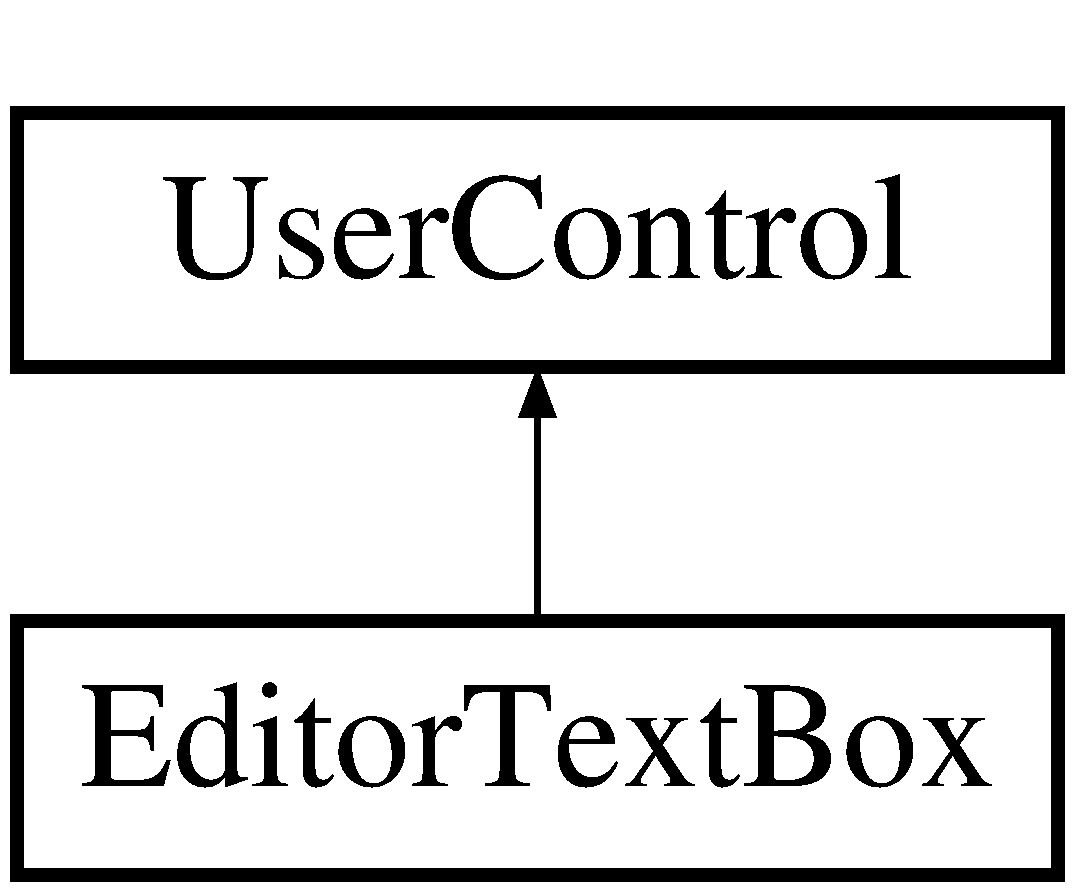
\includegraphics[height=2.000000cm]{classkdz__manager_1_1_editor_text_box}
\end{center}
\end{figure}
\subsubsection*{Открытые члены}
\begin{DoxyCompactItemize}
\item 
{\bf Editor\+Text\+Box} ()
\begin{DoxyCompactList}\small\item\em With this constructor, remember to bind this control before use (call Bind\+To\+Data\+Row\+View) \end{DoxyCompactList}\item 
void {\bf Bind\+To\+Data\+Row\+View} (Data\+Row\+View rowview, string column\+\_\+name)
\begin{DoxyCompactList}\small\item\em Bind this control to Data\+Row\+View object \end{DoxyCompactList}\item 
void {\bf Unbind\+From\+Data} ()
\begin{DoxyCompactList}\small\item\em Resets control properties to default values. This is useful since we can then reuse the controls. \end{DoxyCompactList}\end{DoxyCompactItemize}
\subsubsection*{Статические открытые данные}
\begin{DoxyCompactItemize}
\item 
static Color {\bfseries Success} = Color.\+Light\+Green\label{classkdz__manager_1_1_editor_text_box_a412e64ff5e03578f96baf3d42ca7cc47}

\item 
static Color {\bfseries Failure} = Color.\+Light\+Pink\label{classkdz__manager_1_1_editor_text_box_a66daee56c8498eb96286ff892b941f20}

\item 
static Color {\bfseries Default} = Color.\+White\label{classkdz__manager_1_1_editor_text_box_ae9f7469c1ac140130f288a9a2a417409}

\end{DoxyCompactItemize}
\subsubsection*{Свойства}
\begin{DoxyCompactItemize}
\item 
bool {\bf Binding\+O\+K}\hspace{0.3cm}{\ttfamily  [get, protected set]}
\begin{DoxyCompactList}\small\item\em If we can bind succesfully to the Data\+Table (meaning\+: if the entered data is valid) \end{DoxyCompactList}\item 
string {\bf Label}\hspace{0.3cm}{\ttfamily  [get, set]}
\begin{DoxyCompactList}\small\item\em String to describe the input box \end{DoxyCompactList}\end{DoxyCompactItemize}


\subsubsection{Подробное описание}


См. определение в файле Editor\+Text\+Box.\+cs строка 15



\subsubsection{Конструктор(ы)}
\index{kdz\+\_\+manager\+::\+Editor\+Text\+Box@{kdz\+\_\+manager\+::\+Editor\+Text\+Box}!Editor\+Text\+Box@{Editor\+Text\+Box}}
\index{Editor\+Text\+Box@{Editor\+Text\+Box}!kdz\+\_\+manager\+::\+Editor\+Text\+Box@{kdz\+\_\+manager\+::\+Editor\+Text\+Box}}
\paragraph[{Editor\+Text\+Box()}]{\setlength{\rightskip}{0pt plus 5cm}{\bf Editor\+Text\+Box} (
\begin{DoxyParamCaption}
{}
\end{DoxyParamCaption}
)}\label{classkdz__manager_1_1_editor_text_box_af5312caeb8bdda25f44bd33d20dcbbf8_af5312caeb8bdda25f44bd33d20dcbbf8}


См. определение в файле Editor\+Text\+Box.\+cs строка 40



\subsubsection{Методы}
\index{kdz\+\_\+manager\+::\+Editor\+Text\+Box@{kdz\+\_\+manager\+::\+Editor\+Text\+Box}!Bind\+To\+Data\+Row\+View@{Bind\+To\+Data\+Row\+View}}
\index{Bind\+To\+Data\+Row\+View@{Bind\+To\+Data\+Row\+View}!kdz\+\_\+manager\+::\+Editor\+Text\+Box@{kdz\+\_\+manager\+::\+Editor\+Text\+Box}}
\paragraph[{Bind\+To\+Data\+Row\+View(\+Data\+Row\+View rowview, string column\+\_\+name)}]{\setlength{\rightskip}{0pt plus 5cm}void Bind\+To\+Data\+Row\+View (
\begin{DoxyParamCaption}
\item[{Data\+Row\+View}]{rowview, }
\item[{string}]{column\+\_\+name}
\end{DoxyParamCaption}
)}\label{classkdz__manager_1_1_editor_text_box_a6a04b6bd6845e298aa5c979f64fd48ac_a6a04b6bd6845e298aa5c979f64fd48ac}

\begin{DoxyParams}{Аргументы}
{\em rowview} & \\
\hline
\end{DoxyParams}


См. определение в файле Editor\+Text\+Box.\+cs строка 49

\index{kdz\+\_\+manager\+::\+Editor\+Text\+Box@{kdz\+\_\+manager\+::\+Editor\+Text\+Box}!Unbind\+From\+Data@{Unbind\+From\+Data}}
\index{Unbind\+From\+Data@{Unbind\+From\+Data}!kdz\+\_\+manager\+::\+Editor\+Text\+Box@{kdz\+\_\+manager\+::\+Editor\+Text\+Box}}
\paragraph[{Unbind\+From\+Data()}]{\setlength{\rightskip}{0pt plus 5cm}void Unbind\+From\+Data (
\begin{DoxyParamCaption}
{}
\end{DoxyParamCaption}
)}\label{classkdz__manager_1_1_editor_text_box_a4dbfa2ba7ea7b9f394422a8cf9070df4_a4dbfa2ba7ea7b9f394422a8cf9070df4}


См. определение в файле Editor\+Text\+Box.\+cs строка 102



\subsubsection{Полный список свойств}
\index{kdz\+\_\+manager\+::\+Editor\+Text\+Box@{kdz\+\_\+manager\+::\+Editor\+Text\+Box}!Binding\+O\+K@{Binding\+O\+K}}
\index{Binding\+O\+K@{Binding\+O\+K}!kdz\+\_\+manager\+::\+Editor\+Text\+Box@{kdz\+\_\+manager\+::\+Editor\+Text\+Box}}
\paragraph[{Binding\+O\+K}]{\setlength{\rightskip}{0pt plus 5cm}bool Binding\+O\+K\hspace{0.3cm}{\ttfamily [get]}, {\ttfamily [protected set]}}\label{classkdz__manager_1_1_editor_text_box_a8073b9eea77b0f05bf7286d1baf7933a_a8073b9eea77b0f05bf7286d1baf7933a}


См. определение в файле Editor\+Text\+Box.\+cs строка 25

\index{kdz\+\_\+manager\+::\+Editor\+Text\+Box@{kdz\+\_\+manager\+::\+Editor\+Text\+Box}!Label@{Label}}
\index{Label@{Label}!kdz\+\_\+manager\+::\+Editor\+Text\+Box@{kdz\+\_\+manager\+::\+Editor\+Text\+Box}}
\paragraph[{Label}]{\setlength{\rightskip}{0pt plus 5cm}string Label\hspace{0.3cm}{\ttfamily [get]}, {\ttfamily [set]}}\label{classkdz__manager_1_1_editor_text_box_a0999f1070ce4923004bfb388671f0387_a0999f1070ce4923004bfb388671f0387}


См. определение в файле Editor\+Text\+Box.\+cs строка 31


\subsection{Класс Edit\+Row\+Form}
\label{classkdz__manager_1_1_edit_row_form}\index{Edit\+Row\+Form@{Edit\+Row\+Form}}
Граф наследования\+:Edit\+Row\+Form\+:\begin{figure}[H]
\begin{center}
\leavevmode
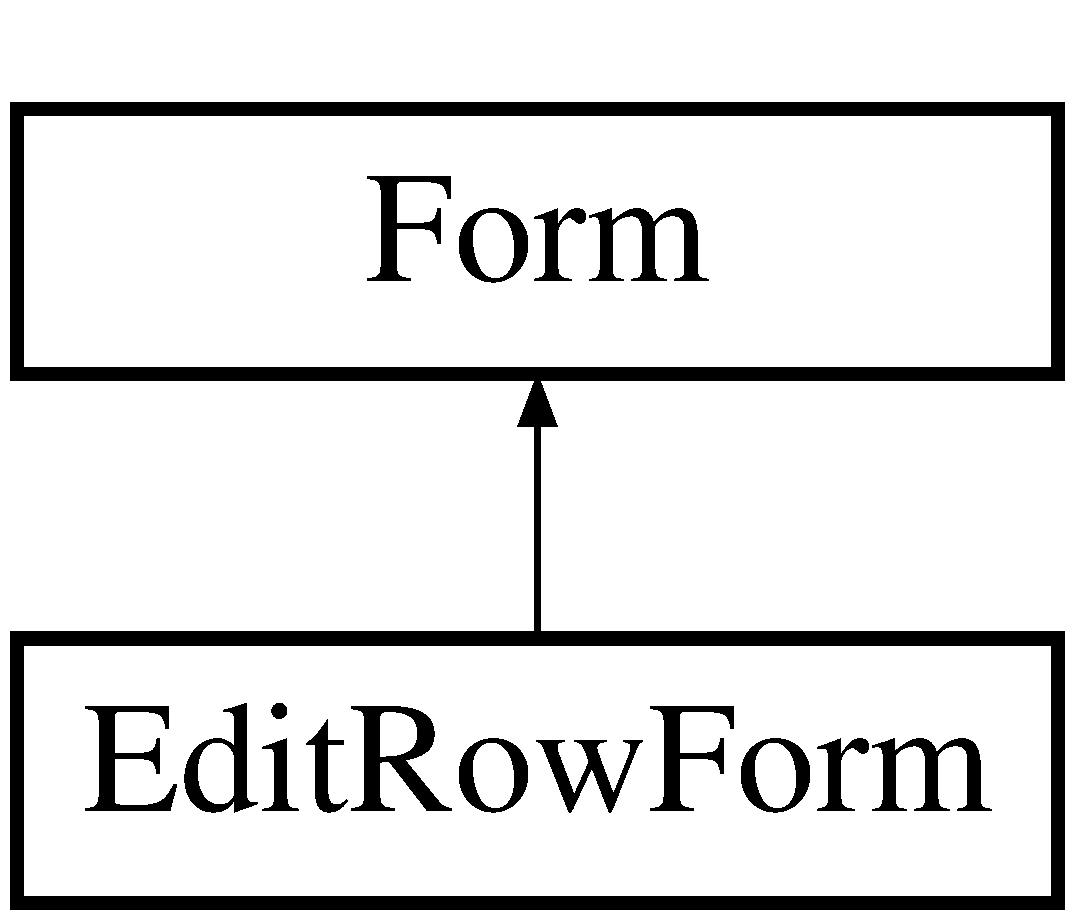
\includegraphics[height=2.000000cm]{classkdz__manager_1_1_edit_row_form}
\end{center}
\end{figure}
\subsubsection*{Открытые члены}
\begin{DoxyCompactItemize}
\item 
{\bfseries Edit\+Row\+Form} (Type rowtype)\label{classkdz__manager_1_1_edit_row_form_a961ae1a89b9f867dba48c197f6ce0f48}

\item 
void {\bf Gen\+List\+Text\+Labels} (Type rowtype)
\begin{DoxyCompactList}\small\item\em Создать поля ввода в зависимости от типа класса. Так один вход поле соответствует классу имущества. \end{DoxyCompactList}\item 
void {\bf Re\+Bind\+Controls\+To\+Data\+Row} (Data\+Row\+View rowview)
\begin{DoxyCompactList}\small\item\em указан текст Входы для отслеживания состояния сетке данных. Это должно позволить пользователю редактировать записи. сбрасывает Data\+Bindings и Back\+Color. необходимо сбросить управления, так как мы повторно использовать их. \end{DoxyCompactList}\end{DoxyCompactItemize}


\subsubsection{Подробное описание}


См. определение в файле Edit\+Row\+Form.\+cs строка 15



\subsubsection{Методы}
\index{kdz\+\_\+manager\+::\+Edit\+Row\+Form@{kdz\+\_\+manager\+::\+Edit\+Row\+Form}!Gen\+List\+Text\+Labels@{Gen\+List\+Text\+Labels}}
\index{Gen\+List\+Text\+Labels@{Gen\+List\+Text\+Labels}!kdz\+\_\+manager\+::\+Edit\+Row\+Form@{kdz\+\_\+manager\+::\+Edit\+Row\+Form}}
\paragraph[{Gen\+List\+Text\+Labels(\+Type rowtype)}]{\setlength{\rightskip}{0pt plus 5cm}void Gen\+List\+Text\+Labels (
\begin{DoxyParamCaption}
\item[{Type}]{rowtype}
\end{DoxyParamCaption}
)}\label{classkdz__manager_1_1_edit_row_form_acd59903c1bfa3bfe7d9d924aa50f2b2a_acd59903c1bfa3bfe7d9d924aa50f2b2a}

\begin{DoxyTemplParams}{Template Parameters}
{\em Type} & The type which should be filled with information.\\
\hline
\end{DoxyTemplParams}


См. определение в файле Edit\+Row\+Form.\+cs строка 32

\index{kdz\+\_\+manager\+::\+Edit\+Row\+Form@{kdz\+\_\+manager\+::\+Edit\+Row\+Form}!Re\+Bind\+Controls\+To\+Data\+Row@{Re\+Bind\+Controls\+To\+Data\+Row}}
\index{Re\+Bind\+Controls\+To\+Data\+Row@{Re\+Bind\+Controls\+To\+Data\+Row}!kdz\+\_\+manager\+::\+Edit\+Row\+Form@{kdz\+\_\+manager\+::\+Edit\+Row\+Form}}
\paragraph[{Re\+Bind\+Controls\+To\+Data\+Row(\+Data\+Row\+View rowview)}]{\setlength{\rightskip}{0pt plus 5cm}void Re\+Bind\+Controls\+To\+Data\+Row (
\begin{DoxyParamCaption}
\item[{Data\+Row\+View}]{rowview}
\end{DoxyParamCaption}
)}\label{classkdz__manager_1_1_edit_row_form_a8f20b30bdd570195fab61c0d08e8ace5_a8f20b30bdd570195fab61c0d08e8ace5}

\begin{DoxyParams}{Аргументы}
{\em rowview} & \\
\hline
\end{DoxyParams}


См. определение в файле Edit\+Row\+Form.\+cs строка 61


\subsection{Шаблон интерфейса I\+From\+Map\+Data\+Row$<$ T $>$}
\label{interfacekdz__manager_1_1_i_from_map_data_row}\index{I\+From\+Map\+Data\+Row$<$ T $>$@{I\+From\+Map\+Data\+Row$<$ T $>$}}
\subsubsection*{Открытые члены}
\begin{DoxyCompactItemize}
\item 
T {\bfseries From\+Map\+Data\+Row} ({\bf Map\+Data\+Row} input)\label{interfacekdz__manager_1_1_i_from_map_data_row_a6bfee7c6ccbd75bb8f757c20752b79f7}

\end{DoxyCompactItemize}


\subsubsection{Подробное описание}


См. определение в файле I\+From\+Map\+Data\+Row.\+cs строка 9


\subsection{Класс Main\+Form}
\label{classkdz__manager_1_1_main_form}\index{Main\+Form@{Main\+Form}}
Граф наследования\+:Main\+Form\+:\begin{figure}[H]
\begin{center}
\leavevmode
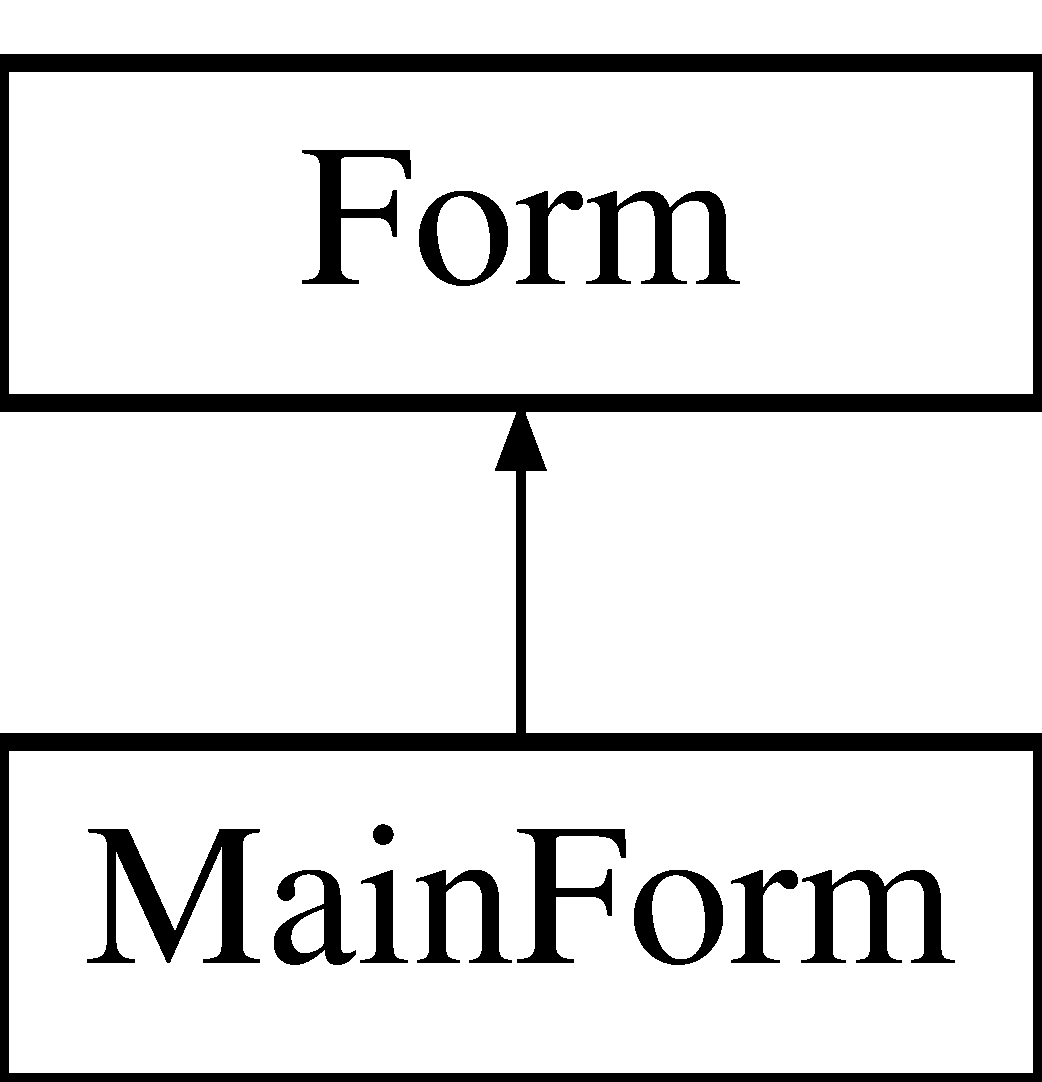
\includegraphics[height=2.000000cm]{classkdz__manager_1_1_main_form}
\end{center}
\end{figure}


\subsubsection{Подробное описание}


См. определение в файле Form1.\+cs строка 18


\subsection{Класс Map\+Data\+Row}
\label{classkdz__manager_1_1_map_data_row}\index{Map\+Data\+Row@{Map\+Data\+Row}}


Карты одна строка в C\+S\+V файл со свойствами.  


\subsubsection*{Открытые члены}
\begin{DoxyCompactItemize}
\item 
{\bf Map\+Data\+Row} ()
\begin{DoxyCompactList}\small\item\em Беспараметрическая конструктор, необходимые для использования в C\+S\+V парсер. \end{DoxyCompactList}\end{DoxyCompactItemize}
\subsubsection*{Свойства}
\begin{DoxyCompactItemize}
\item 
int {\bfseries R\+O\+W\+N\+U\+M}\hspace{0.3cm}{\ttfamily  [get, set]}\label{classkdz__manager_1_1_map_data_row_a4d8b0af11d5d24e4fe27acb051dd68c0}

\item 
string {\bfseries Common\+Name}\hspace{0.3cm}{\ttfamily  [get, set]}\label{classkdz__manager_1_1_map_data_row_aaddc6d183e79d64b80b4ace5c2495e9b}

\item 
string {\bfseries Full\+Name}\hspace{0.3cm}{\ttfamily  [get, set]}\label{classkdz__manager_1_1_map_data_row_a2c9bf07e0f7c919dfede2f09728bd334}

\item 
string {\bfseries Short\+Name}\hspace{0.3cm}{\ttfamily  [get, set]}\label{classkdz__manager_1_1_map_data_row_a3a016153fc0223aafe80091ff4e5ceac}

\item 
string {\bfseries Adm\+Area\+Code}\hspace{0.3cm}{\ttfamily  [get, set]}\label{classkdz__manager_1_1_map_data_row_ab7eb47ebdd8dc4601e798df1860a76d4}

\item 
string {\bfseries Adm\+Area}\hspace{0.3cm}{\ttfamily  [get, set]}\label{classkdz__manager_1_1_map_data_row_a681cc5993f19cb1ddf82a5d7f139f724}

\item 
string {\bfseries District}\hspace{0.3cm}{\ttfamily  [get, set]}\label{classkdz__manager_1_1_map_data_row_a15bedb0529df8935aa4c0086e6bccc7b}

\item 
string {\bfseries Postal\+Code}\hspace{0.3cm}{\ttfamily  [get, set]}\label{classkdz__manager_1_1_map_data_row_a66adf95f43e33ffbc2414d100c06a7cf}

\item 
string {\bfseries Address}\hspace{0.3cm}{\ttfamily  [get, set]}\label{classkdz__manager_1_1_map_data_row_aec57182df53b04aceca477433c48ecfc}

\item 
string {\bfseries Nearest\+Metro\+Stations}\hspace{0.3cm}{\ttfamily  [get, set]}\label{classkdz__manager_1_1_map_data_row_a290d8b82d3925cd0435491be2782d7be}

\item 
string {\bfseries Chief\+Name}\hspace{0.3cm}{\ttfamily  [get, set]}\label{classkdz__manager_1_1_map_data_row_a2b949c4066c7da75ac75b9e4c43269d3}

\item 
string {\bfseries Chief\+Position}\hspace{0.3cm}{\ttfamily  [get, set]}\label{classkdz__manager_1_1_map_data_row_ab744770e144d24909e9ed3f50748843e}

\item 
string {\bfseries Chief\+Phone}\hspace{0.3cm}{\ttfamily  [get, set]}\label{classkdz__manager_1_1_map_data_row_a64ef3ef40186d005d587d77c70918067}

\item 
string {\bfseries Contact\+Phone}\hspace{0.3cm}{\ttfamily  [get, set]}\label{classkdz__manager_1_1_map_data_row_a60e6463566cb751d141d67d7984f3172}

\item 
string {\bfseries Archive\+Phone}\hspace{0.3cm}{\ttfamily  [get, set]}\label{classkdz__manager_1_1_map_data_row_ac0123ac2ba612e4e6639c3be12fa0b38}

\item 
string {\bfseries Sign\+P\+G\+U}\hspace{0.3cm}{\ttfamily  [get, set]}\label{classkdz__manager_1_1_map_data_row_a830f3a9d060596330cb0a05e16585d08}

\item 
string {\bfseries Working\+Hours}\hspace{0.3cm}{\ttfamily  [get, set]}\label{classkdz__manager_1_1_map_data_row_ae23dd44a8a4e9b18cff4494ecf4d03cc}

\item 
string {\bfseries Clarification\+Of\+Working\+Hours}\hspace{0.3cm}{\ttfamily  [get, set]}\label{classkdz__manager_1_1_map_data_row_a201b25d204d2985fae8cabbfa1dd2c6e}

\item 
string {\bfseries Web\+Site}\hspace{0.3cm}{\ttfamily  [get, set]}\label{classkdz__manager_1_1_map_data_row_adb0ed212a01483827640afd66235aa28}

\item 
float {\bfseries X\+\_\+\+W\+G\+S}\hspace{0.3cm}{\ttfamily  [get, set]}\label{classkdz__manager_1_1_map_data_row_affa3a219101796e0b7970061b4688790}

\item 
float {\bfseries Y\+\_\+\+W\+G\+S}\hspace{0.3cm}{\ttfamily  [get, set]}\label{classkdz__manager_1_1_map_data_row_afe838c8f7955c7af682c53bc1147d698}

\item 
string {\bfseries G\+L\+O\+B\+A\+L\+I\+D}\hspace{0.3cm}{\ttfamily  [get, set]}\label{classkdz__manager_1_1_map_data_row_a3455001407f0d47c030d9f6023314c04}

\end{DoxyCompactItemize}


\subsubsection{Подробное описание}


См. определение в файле Map\+Data\+Row.\+cs строка 12



\subsubsection{Конструктор(ы)}
\index{kdz\+\_\+manager\+::\+Map\+Data\+Row@{kdz\+\_\+manager\+::\+Map\+Data\+Row}!Map\+Data\+Row@{Map\+Data\+Row}}
\index{Map\+Data\+Row@{Map\+Data\+Row}!kdz\+\_\+manager\+::\+Map\+Data\+Row@{kdz\+\_\+manager\+::\+Map\+Data\+Row}}
\paragraph[{Map\+Data\+Row()}]{\setlength{\rightskip}{0pt plus 5cm}{\bf Map\+Data\+Row} (
\begin{DoxyParamCaption}
{}
\end{DoxyParamCaption}
)}\label{classkdz__manager_1_1_map_data_row_ad6ac503f8eacb1dc68817e11004bab19_ad6ac503f8eacb1dc68817e11004bab19}


См. определение в файле Map\+Data\+Row.\+cs строка 40


\subsection{Класс Open\+Data}
\label{classkdz__manager_1_1_open_data}\index{Open\+Data@{Open\+Data}}
\subsubsection*{Открытые члены}
\begin{DoxyCompactItemize}
\item 
void {\bf Parse\+As\+Map\+Data\+C\+S\+V} (string filepath)
\begin{DoxyCompactList}\small\item\em Open file, read and verify data, make data table and run control intialisations. \end{DoxyCompactList}\item 
void {\bf Update\+Dynamic\+Column\+On\+Row\+Edit} (Data\+Table dt, Data\+Row oldrow, Data\+Row newrow)
\begin{DoxyCompactList}\small\item\em Recalculates the dynamic column for the row. \end{DoxyCompactList}\item 
void {\bf Import\+Processing} ()
\begin{DoxyCompactList}\small\item\em Function to fill Inner and Outer Lists based on data in Raw list. \end{DoxyCompactList}\item 
Data\+Table {\bf To\+Data\+Table$<$ T $>$} (I\+List$<$ T $>$ data)
\begin{DoxyCompactList}\small\item\em Read through the properties of T and assemble a Data\+Table that would represent it. \end{DoxyCompactList}\item 
Data\+Table {\bf Empty\+Table\+From\+Type$<$ T $>$} ()
\begin{DoxyCompactList}\small\item\em Make an empty data table with layout to contain type T. \end{DoxyCompactList}\end{DoxyCompactItemize}
\subsubsection*{Открытые статические члены}
\begin{DoxyCompactItemize}
\item 
static string {\bf Open\+File\+Dialog\+Get\+Path} ()
\begin{DoxyCompactList}\small\item\em Opens a dialog to get path of file to open from te user. \end{DoxyCompactList}\end{DoxyCompactItemize}
\subsubsection*{Открытые атрибуты}
\begin{DoxyCompactItemize}
\item 
List$<$ {\bf Registry\+Office\+Data\+Row} $>$ {\bf Inner}
\begin{DoxyCompactList}\small\item\em Simple type. \end{DoxyCompactList}\item 
List$<$ {\bf Admin\+Area\+Data\+Row} $>$ {\bf Outer}
\begin{DoxyCompactList}\small\item\em Advanced type that aggregates simple types. \end{DoxyCompactList}\item 
List$<$ {\bf Map\+Data\+Row} $>$ {\bf Raw}
\begin{DoxyCompactList}\small\item\em Result of parsing C\+S\+V file \end{DoxyCompactList}\item 
string {\bfseries Outer2\+Inner\+Qty\+Dynamic\+Column} = \char`\"{}Regions\+In\+Adm\+Area\char`\"{}\label{classkdz__manager_1_1_open_data_a93728bb726e51b49493c8628f2037c94}

\item 
string {\bfseries Outer\+Key\+Column} = \char`\"{}Adm\+Area\+Code\char`\"{}\label{classkdz__manager_1_1_open_data_a8190edc858cdfea68fb72782608ea6f8}

\item 
string {\bfseries Filter\+Adm\+Area} = \char`\"{}Adm\+Area\char`\"{}\label{classkdz__manager_1_1_open_data_a5fc102f36a819b3bc81627a8d931ab3e}

\item 
string {\bfseries Filter\+Adm\+Area\+Code} = \char`\"{}Adm\+Area\+Code\char`\"{}\label{classkdz__manager_1_1_open_data_afd6b740ac445668267e4f69729b7d391}

\end{DoxyCompactItemize}


\subsubsection{Подробное описание}


См. определение в файле Open\+Data.\+cs строка 306



\subsubsection{Методы}
\index{kdz\+\_\+manager\+::\+Open\+Data@{kdz\+\_\+manager\+::\+Open\+Data}!Empty\+Table\+From\+Type$<$ T $>$@{Empty\+Table\+From\+Type$<$ T $>$}}
\index{Empty\+Table\+From\+Type$<$ T $>$@{Empty\+Table\+From\+Type$<$ T $>$}!kdz\+\_\+manager\+::\+Open\+Data@{kdz\+\_\+manager\+::\+Open\+Data}}
\paragraph[{Empty\+Table\+From\+Type$<$ T $>$()}]{\setlength{\rightskip}{0pt plus 5cm}Data\+Table Empty\+Table\+From\+Type$<$ T $>$ (
\begin{DoxyParamCaption}
{}
\end{DoxyParamCaption}
)}\label{classkdz__manager_1_1_open_data_a92775521c23e5242e0266086338c4ef6_a92775521c23e5242e0266086338c4ef6}

\begin{DoxyTemplParams}{Template Parameters}
{\em T} & \\
\hline
\end{DoxyTemplParams}

\begin{DoxyParams}{Аргументы}
{\em data} & \\
\hline
\end{DoxyParams}
\begin{DoxyReturn}{Возвращает}

\end{DoxyReturn}


См. определение в файле Open\+Data.\+cs строка 464

\index{kdz\+\_\+manager\+::\+Open\+Data@{kdz\+\_\+manager\+::\+Open\+Data}!Import\+Processing@{Import\+Processing}}
\index{Import\+Processing@{Import\+Processing}!kdz\+\_\+manager\+::\+Open\+Data@{kdz\+\_\+manager\+::\+Open\+Data}}
\paragraph[{Import\+Processing()}]{\setlength{\rightskip}{0pt plus 5cm}void Import\+Processing (
\begin{DoxyParamCaption}
{}
\end{DoxyParamCaption}
)}\label{classkdz__manager_1_1_open_data_ae25690f340153fc869429ee913b711bd_ae25690f340153fc869429ee913b711bd}


См. определение в файле Open\+Data.\+cs строка 399

\index{kdz\+\_\+manager\+::\+Open\+Data@{kdz\+\_\+manager\+::\+Open\+Data}!Open\+File\+Dialog\+Get\+Path@{Open\+File\+Dialog\+Get\+Path}}
\index{Open\+File\+Dialog\+Get\+Path@{Open\+File\+Dialog\+Get\+Path}!kdz\+\_\+manager\+::\+Open\+Data@{kdz\+\_\+manager\+::\+Open\+Data}}
\paragraph[{Open\+File\+Dialog\+Get\+Path()}]{\setlength{\rightskip}{0pt plus 5cm}static string Open\+File\+Dialog\+Get\+Path (
\begin{DoxyParamCaption}
{}
\end{DoxyParamCaption}
)\hspace{0.3cm}{\ttfamily [static]}}\label{classkdz__manager_1_1_open_data_a9d5c1006b3d1e0c9bcef28e7b0283fda_a9d5c1006b3d1e0c9bcef28e7b0283fda}
\begin{DoxyReturn}{Возвращает}

\end{DoxyReturn}


См. определение в файле Open\+Data.\+cs строка 480

\index{kdz\+\_\+manager\+::\+Open\+Data@{kdz\+\_\+manager\+::\+Open\+Data}!Parse\+As\+Map\+Data\+C\+S\+V@{Parse\+As\+Map\+Data\+C\+S\+V}}
\index{Parse\+As\+Map\+Data\+C\+S\+V@{Parse\+As\+Map\+Data\+C\+S\+V}!kdz\+\_\+manager\+::\+Open\+Data@{kdz\+\_\+manager\+::\+Open\+Data}}
\paragraph[{Parse\+As\+Map\+Data\+C\+S\+V(string filepath)}]{\setlength{\rightskip}{0pt plus 5cm}void Parse\+As\+Map\+Data\+C\+S\+V (
\begin{DoxyParamCaption}
\item[{string}]{filepath}
\end{DoxyParamCaption}
)}\label{classkdz__manager_1_1_open_data_a36bd09dfa54a1139e116b9baf7d0fd45_a36bd09dfa54a1139e116b9baf7d0fd45}

\begin{DoxyParams}{Аргументы}
{\em filepath} & \\
\hline
\end{DoxyParams}
\begin{DoxyReturn}{Возвращает}

\end{DoxyReturn}


См. определение в файле Open\+Data.\+cs строка 342

\index{kdz\+\_\+manager\+::\+Open\+Data@{kdz\+\_\+manager\+::\+Open\+Data}!To\+Data\+Table$<$ T $>$@{To\+Data\+Table$<$ T $>$}}
\index{To\+Data\+Table$<$ T $>$@{To\+Data\+Table$<$ T $>$}!kdz\+\_\+manager\+::\+Open\+Data@{kdz\+\_\+manager\+::\+Open\+Data}}
\paragraph[{To\+Data\+Table$<$ T $>$(\+I\+List$<$ T $>$ data)}]{\setlength{\rightskip}{0pt plus 5cm}Data\+Table To\+Data\+Table$<$ T $>$ (
\begin{DoxyParamCaption}
\item[{I\+List$<$ T $>$}]{data}
\end{DoxyParamCaption}
)}\label{classkdz__manager_1_1_open_data_ab27f76fc2774c51bfd4cd5e03d25ff16_ab27f76fc2774c51bfd4cd5e03d25ff16}

\begin{DoxyTemplParams}{Template Parameters}
{\em T} & \\
\hline
\end{DoxyTemplParams}

\begin{DoxyParams}{Аргументы}
{\em data} & \\
\hline
\end{DoxyParams}
\begin{DoxyReturn}{Возвращает}

\end{DoxyReturn}


См. определение в файле Open\+Data.\+cs строка 436

\index{kdz\+\_\+manager\+::\+Open\+Data@{kdz\+\_\+manager\+::\+Open\+Data}!Update\+Dynamic\+Column\+On\+Row\+Edit@{Update\+Dynamic\+Column\+On\+Row\+Edit}}
\index{Update\+Dynamic\+Column\+On\+Row\+Edit@{Update\+Dynamic\+Column\+On\+Row\+Edit}!kdz\+\_\+manager\+::\+Open\+Data@{kdz\+\_\+manager\+::\+Open\+Data}}
\paragraph[{Update\+Dynamic\+Column\+On\+Row\+Edit(\+Data\+Table dt, Data\+Row oldrow, Data\+Row newrow)}]{\setlength{\rightskip}{0pt plus 5cm}void Update\+Dynamic\+Column\+On\+Row\+Edit (
\begin{DoxyParamCaption}
\item[{Data\+Table}]{dt, }
\item[{Data\+Row}]{oldrow, }
\item[{Data\+Row}]{newrow}
\end{DoxyParamCaption}
)}\label{classkdz__manager_1_1_open_data_a6399c5b40ed128a5012b87773d630ce6_a6399c5b40ed128a5012b87773d630ce6}

\begin{DoxyParams}{Аргументы}
{\em dt} & \\
\hline
{\em oldrow} & \\
\hline
{\em newrow} & \\
\hline
\end{DoxyParams}


См. определение в файле Open\+Data.\+cs строка 360



\subsubsection{Данные класса}
\index{kdz\+\_\+manager\+::\+Open\+Data@{kdz\+\_\+manager\+::\+Open\+Data}!Inner@{Inner}}
\index{Inner@{Inner}!kdz\+\_\+manager\+::\+Open\+Data@{kdz\+\_\+manager\+::\+Open\+Data}}
\paragraph[{Inner}]{\setlength{\rightskip}{0pt plus 5cm}List$<${\bf Registry\+Office\+Data\+Row}$>$ Inner}\label{classkdz__manager_1_1_open_data_a4a48764400c4991c8b0c82ab12e191e6_a4a48764400c4991c8b0c82ab12e191e6}


См. определение в файле Open\+Data.\+cs строка 312

\index{kdz\+\_\+manager\+::\+Open\+Data@{kdz\+\_\+manager\+::\+Open\+Data}!Outer@{Outer}}
\index{Outer@{Outer}!kdz\+\_\+manager\+::\+Open\+Data@{kdz\+\_\+manager\+::\+Open\+Data}}
\paragraph[{Outer}]{\setlength{\rightskip}{0pt plus 5cm}List$<${\bf Admin\+Area\+Data\+Row}$>$ Outer}\label{classkdz__manager_1_1_open_data_af87c250148a042bdc1abafe9273c25ce_af87c250148a042bdc1abafe9273c25ce}


См. определение в файле Open\+Data.\+cs строка 316

\index{kdz\+\_\+manager\+::\+Open\+Data@{kdz\+\_\+manager\+::\+Open\+Data}!Raw@{Raw}}
\index{Raw@{Raw}!kdz\+\_\+manager\+::\+Open\+Data@{kdz\+\_\+manager\+::\+Open\+Data}}
\paragraph[{Raw}]{\setlength{\rightskip}{0pt plus 5cm}List$<${\bf Map\+Data\+Row}$>$ Raw}\label{classkdz__manager_1_1_open_data_aaa7963fb899e3dafb354bb287c7156c7_aaa7963fb899e3dafb354bb287c7156c7}


См. определение в файле Open\+Data.\+cs строка 320


\subsection{Класс Program}
\label{classkdz__manager_1_1_program}\index{Program@{Program}}


\subsubsection{Подробное описание}


См. определение в файле Program.\+cs строка 32


\subsection{Класс Recent\+Files\+Folders}
\label{classkdz__manager_1_1_recent_files_folders}\index{Recent\+Files\+Folders@{Recent\+Files\+Folders}}
\subsubsection*{Открытые члены}
\begin{DoxyCompactItemize}
\item 
{\bf Recent\+Files\+Folders} ()
\item 
void {\bf Replace\+Open\+Recent\+Menu} (Tool\+Strip\+Menu\+Item open\+\_\+recent\+\_\+menu, Action$<$ string $>$ onclick)
\begin{DoxyCompactList}\small\item\em The Open\+Recent files have changed. Refresh the view in menu. \end{DoxyCompactList}\item 
void {\bf Add\+Recent\+File} (string file)
\begin{DoxyCompactList}\small\item\em Add a new item to the Recent-\/\+Files menu and save it persistently \end{DoxyCompactList}\end{DoxyCompactItemize}
\subsubsection*{Свойства}
\begin{DoxyCompactItemize}
\item 
string {\bfseries Currently\+Open\+File\+Path}\hspace{0.3cm}{\ttfamily  [get, set]}\label{classkdz__manager_1_1_recent_files_folders_a69ecdef3984e3864eec1ad459bc98161}

\end{DoxyCompactItemize}
\subsubsection*{События}
\begin{DoxyCompactItemize}
\item 
Action$<$ string $>$ {\bf Currently\+Open\+File\+Path\+Changed}
\begin{DoxyCompactList}\small\item\em Event to fire on current filepath change. \end{DoxyCompactList}\end{DoxyCompactItemize}


\subsubsection{Подробное описание}


См. определение в файле Recent\+Files\+Folders.\+cs строка 18



\subsubsection{Конструктор(ы)}
\index{kdz\+\_\+manager\+::\+Recent\+Files\+Folders@{kdz\+\_\+manager\+::\+Recent\+Files\+Folders}!Recent\+Files\+Folders@{Recent\+Files\+Folders}}
\index{Recent\+Files\+Folders@{Recent\+Files\+Folders}!kdz\+\_\+manager\+::\+Recent\+Files\+Folders@{kdz\+\_\+manager\+::\+Recent\+Files\+Folders}}
\paragraph[{Recent\+Files\+Folders()}]{\setlength{\rightskip}{0pt plus 5cm}{\bf Recent\+Files\+Folders} (
\begin{DoxyParamCaption}
{}
\end{DoxyParamCaption}
)}\label{classkdz__manager_1_1_recent_files_folders_a8828d6fa536ace9dcf00589d4a40e940_a8828d6fa536ace9dcf00589d4a40e940}
Set sensible value for directory in Open\+File dialog. 

См. определение в файле Recent\+Files\+Folders.\+cs строка 36



\subsubsection{Методы}
\index{kdz\+\_\+manager\+::\+Recent\+Files\+Folders@{kdz\+\_\+manager\+::\+Recent\+Files\+Folders}!Add\+Recent\+File@{Add\+Recent\+File}}
\index{Add\+Recent\+File@{Add\+Recent\+File}!kdz\+\_\+manager\+::\+Recent\+Files\+Folders@{kdz\+\_\+manager\+::\+Recent\+Files\+Folders}}
\paragraph[{Add\+Recent\+File(string file)}]{\setlength{\rightskip}{0pt plus 5cm}void Add\+Recent\+File (
\begin{DoxyParamCaption}
\item[{string}]{file}
\end{DoxyParamCaption}
)}\label{classkdz__manager_1_1_recent_files_folders_ac3524f09b3d54d66da8bcbc186ee4e26_ac3524f09b3d54d66da8bcbc186ee4e26}

\begin{DoxyParams}{Аргументы}
{\em file} & \\
\hline
\end{DoxyParams}


См. определение в файле Recent\+Files\+Folders.\+cs строка 74

\index{kdz\+\_\+manager\+::\+Recent\+Files\+Folders@{kdz\+\_\+manager\+::\+Recent\+Files\+Folders}!Replace\+Open\+Recent\+Menu@{Replace\+Open\+Recent\+Menu}}
\index{Replace\+Open\+Recent\+Menu@{Replace\+Open\+Recent\+Menu}!kdz\+\_\+manager\+::\+Recent\+Files\+Folders@{kdz\+\_\+manager\+::\+Recent\+Files\+Folders}}
\paragraph[{Replace\+Open\+Recent\+Menu(\+Tool\+Strip\+Menu\+Item open\+\_\+recent\+\_\+menu, Action$<$ string $>$ onclick)}]{\setlength{\rightskip}{0pt plus 5cm}void Replace\+Open\+Recent\+Menu (
\begin{DoxyParamCaption}
\item[{Tool\+Strip\+Menu\+Item}]{open\+\_\+recent\+\_\+menu, }
\item[{Action$<$ string $>$}]{onclick}
\end{DoxyParamCaption}
)}\label{classkdz__manager_1_1_recent_files_folders_a6dd09b7928c3f40d9fac4e695d4e33ff_a6dd09b7928c3f40d9fac4e695d4e33ff}


См. определение в файле Recent\+Files\+Folders.\+cs строка 54



\subsubsection{Cобытия}
\index{kdz\+\_\+manager\+::\+Recent\+Files\+Folders@{kdz\+\_\+manager\+::\+Recent\+Files\+Folders}!Currently\+Open\+File\+Path\+Changed@{Currently\+Open\+File\+Path\+Changed}}
\index{Currently\+Open\+File\+Path\+Changed@{Currently\+Open\+File\+Path\+Changed}!kdz\+\_\+manager\+::\+Recent\+Files\+Folders@{kdz\+\_\+manager\+::\+Recent\+Files\+Folders}}
\paragraph[{Currently\+Open\+File\+Path\+Changed}]{\setlength{\rightskip}{0pt plus 5cm}Action$<$ string$>$ Currently\+Open\+File\+Path\+Changed}\label{classkdz__manager_1_1_recent_files_folders_a1a14591e1525a82f18f4ca1f6621fd00_a1a14591e1525a82f18f4ca1f6621fd00}


См. определение в файле Recent\+Files\+Folders.\+cs строка 33


\subsection{Класс Registry\+Office\+Data\+Row}
\label{classkdz__manager_1_1_registry_office_data_row}\index{Registry\+Office\+Data\+Row@{Registry\+Office\+Data\+Row}}


Represents some books.  


Граф наследования\+:Registry\+Office\+Data\+Row\+:\begin{figure}[H]
\begin{center}
\leavevmode
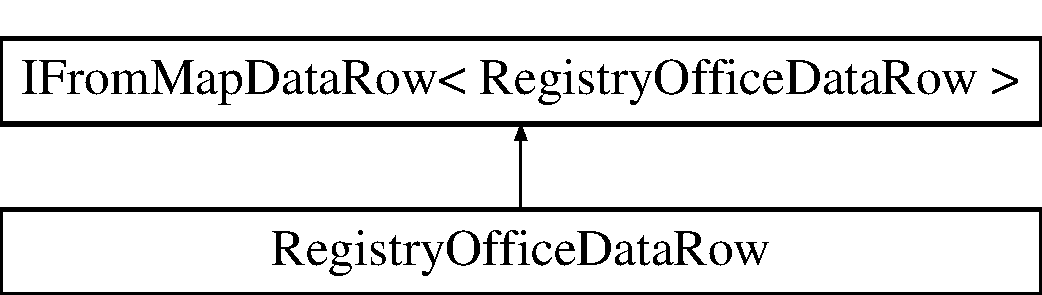
\includegraphics[height=2.000000cm]{classkdz__manager_1_1_registry_office_data_row}
\end{center}
\end{figure}
\subsubsection*{Открытые члены}
\begin{DoxyCompactItemize}
\item 
{\bf Registry\+Office\+Data\+Row} ()
\begin{DoxyCompactList}\small\item\em Parameterless constructor necessary for use in C\+S\+V parser. \end{DoxyCompactList}\item 
{\bf Registry\+Office\+Data\+Row} ({\bf Map\+Data\+Row} input)
\begin{DoxyCompactList}\small\item\em Make from Map data raw \end{DoxyCompactList}\item 
{\bf Registry\+Office\+Data\+Row} {\bf From\+Map\+Data\+Row} ({\bf Map\+Data\+Row} input)
\begin{DoxyCompactList}\small\item\em Create new instance from parsed data \end{DoxyCompactList}\end{DoxyCompactItemize}
\subsubsection*{Свойства}
\begin{DoxyCompactItemize}
\item 
int {\bfseries R\+O\+W\+N\+U\+M}\hspace{0.3cm}{\ttfamily  [get, set]}\label{classkdz__manager_1_1_registry_office_data_row_a4d8b0af11d5d24e4fe27acb051dd68c0}

\item 
string {\bfseries Common\+Name}\hspace{0.3cm}{\ttfamily  [get, set]}\label{classkdz__manager_1_1_registry_office_data_row_aaddc6d183e79d64b80b4ace5c2495e9b}

\item 
string {\bfseries Full\+Name}\hspace{0.3cm}{\ttfamily  [get, set]}\label{classkdz__manager_1_1_registry_office_data_row_a2c9bf07e0f7c919dfede2f09728bd334}

\item 
string {\bfseries Short\+Name}\hspace{0.3cm}{\ttfamily  [get, set]}\label{classkdz__manager_1_1_registry_office_data_row_a3a016153fc0223aafe80091ff4e5ceac}

\item 
string {\bfseries District}\hspace{0.3cm}{\ttfamily  [get, set]}\label{classkdz__manager_1_1_registry_office_data_row_a15bedb0529df8935aa4c0086e6bccc7b}

\item 
string {\bfseries Postal\+Code}\hspace{0.3cm}{\ttfamily  [get, set]}\label{classkdz__manager_1_1_registry_office_data_row_a66adf95f43e33ffbc2414d100c06a7cf}

\item 
string {\bfseries Address}\hspace{0.3cm}{\ttfamily  [get, set]}\label{classkdz__manager_1_1_registry_office_data_row_aec57182df53b04aceca477433c48ecfc}

\item 
string {\bfseries Nearest\+Metro\+Stations}\hspace{0.3cm}{\ttfamily  [get, set]}\label{classkdz__manager_1_1_registry_office_data_row_a290d8b82d3925cd0435491be2782d7be}

\item 
string {\bfseries Chief\+Name}\hspace{0.3cm}{\ttfamily  [get, set]}\label{classkdz__manager_1_1_registry_office_data_row_a2b949c4066c7da75ac75b9e4c43269d3}

\item 
string {\bfseries Chief\+Position}\hspace{0.3cm}{\ttfamily  [get, set]}\label{classkdz__manager_1_1_registry_office_data_row_ab744770e144d24909e9ed3f50748843e}

\item 
string {\bfseries Chief\+Phone}\hspace{0.3cm}{\ttfamily  [get, set]}\label{classkdz__manager_1_1_registry_office_data_row_a64ef3ef40186d005d587d77c70918067}

\item 
string {\bfseries Contact\+Phone}\hspace{0.3cm}{\ttfamily  [get, set]}\label{classkdz__manager_1_1_registry_office_data_row_a60e6463566cb751d141d67d7984f3172}

\item 
string {\bfseries Archive\+Phone}\hspace{0.3cm}{\ttfamily  [get, set]}\label{classkdz__manager_1_1_registry_office_data_row_ac0123ac2ba612e4e6639c3be12fa0b38}

\item 
string {\bfseries Sign\+P\+G\+U}\hspace{0.3cm}{\ttfamily  [get, set]}\label{classkdz__manager_1_1_registry_office_data_row_a830f3a9d060596330cb0a05e16585d08}

\item 
string {\bfseries Working\+Hours}\hspace{0.3cm}{\ttfamily  [get, set]}\label{classkdz__manager_1_1_registry_office_data_row_ae23dd44a8a4e9b18cff4494ecf4d03cc}

\item 
string {\bfseries Clarification\+Of\+Working\+Hours}\hspace{0.3cm}{\ttfamily  [get, set]}\label{classkdz__manager_1_1_registry_office_data_row_a201b25d204d2985fae8cabbfa1dd2c6e}

\item 
string {\bfseries Web\+Site}\hspace{0.3cm}{\ttfamily  [get, set]}\label{classkdz__manager_1_1_registry_office_data_row_adb0ed212a01483827640afd66235aa28}

\item 
float {\bfseries X\+\_\+\+W\+G\+S}\hspace{0.3cm}{\ttfamily  [get, set]}\label{classkdz__manager_1_1_registry_office_data_row_affa3a219101796e0b7970061b4688790}

\item 
float {\bfseries Y\+\_\+\+W\+G\+S}\hspace{0.3cm}{\ttfamily  [get, set]}\label{classkdz__manager_1_1_registry_office_data_row_afe838c8f7955c7af682c53bc1147d698}

\item 
string {\bfseries G\+L\+O\+B\+A\+L\+I\+D}\hspace{0.3cm}{\ttfamily  [get, set]}\label{classkdz__manager_1_1_registry_office_data_row_a3455001407f0d47c030d9f6023314c04}

\end{DoxyCompactItemize}


\subsubsection{Подробное описание}


См. определение в файле Registry\+Office\+Data\+Row.\+cs строка 12



\subsubsection{Конструктор(ы)}
\index{kdz\+\_\+manager\+::\+Registry\+Office\+Data\+Row@{kdz\+\_\+manager\+::\+Registry\+Office\+Data\+Row}!Registry\+Office\+Data\+Row@{Registry\+Office\+Data\+Row}}
\index{Registry\+Office\+Data\+Row@{Registry\+Office\+Data\+Row}!kdz\+\_\+manager\+::\+Registry\+Office\+Data\+Row@{kdz\+\_\+manager\+::\+Registry\+Office\+Data\+Row}}
\paragraph[{Registry\+Office\+Data\+Row}]{\setlength{\rightskip}{0pt plus 5cm}{\bf Registry\+Office\+Data\+Row} (
\begin{DoxyParamCaption}
{}
\end{DoxyParamCaption}
)}\label{classkdz__manager_1_1_registry_office_data_row_a4e51d6eb2c0f1f4ab3fdee6d60bbbd47_a4e51d6eb2c0f1f4ab3fdee6d60bbbd47}


См. определение в файле Registry\+Office\+Data\+Row.\+cs строка 40

\index{kdz\+\_\+manager\+::\+Registry\+Office\+Data\+Row@{kdz\+\_\+manager\+::\+Registry\+Office\+Data\+Row}!Registry\+Office\+Data\+Row@{Registry\+Office\+Data\+Row}}
\index{Registry\+Office\+Data\+Row@{Registry\+Office\+Data\+Row}!kdz\+\_\+manager\+::\+Registry\+Office\+Data\+Row@{kdz\+\_\+manager\+::\+Registry\+Office\+Data\+Row}}
\paragraph[{Registry\+Office\+Data\+Row}]{\setlength{\rightskip}{0pt plus 5cm}{\bf Registry\+Office\+Data\+Row} (
\begin{DoxyParamCaption}
\item[{{\bf Map\+Data\+Row}}]{input}
\end{DoxyParamCaption}
)}\label{classkdz__manager_1_1_registry_office_data_row_a896cdb16fdb97b22709f69795bd2e138_a896cdb16fdb97b22709f69795bd2e138}

\begin{DoxyParams}{Аргументы}
{\em input} & Original object to deep copy from.\\
\hline
\end{DoxyParams}


См. определение в файле Registry\+Office\+Data\+Row.\+cs строка 70



\subsubsection{Методы}
\index{kdz\+\_\+manager\+::\+Registry\+Office\+Data\+Row@{kdz\+\_\+manager\+::\+Registry\+Office\+Data\+Row}!From\+Map\+Data\+Row@{From\+Map\+Data\+Row}}
\index{From\+Map\+Data\+Row@{From\+Map\+Data\+Row}!kdz\+\_\+manager\+::\+Registry\+Office\+Data\+Row@{kdz\+\_\+manager\+::\+Registry\+Office\+Data\+Row}}
\paragraph[{From\+Map\+Data\+Row}]{\setlength{\rightskip}{0pt plus 5cm}{\bf Registry\+Office\+Data\+Row} From\+Map\+Data\+Row (
\begin{DoxyParamCaption}
\item[{{\bf Map\+Data\+Row}}]{input}
\end{DoxyParamCaption}
)}\label{classkdz__manager_1_1_registry_office_data_row_a87bc75e1b2b9a7161f58cba0739c93a8_a87bc75e1b2b9a7161f58cba0739c93a8}
\begin{DoxyReturn}{Возвращает}

\end{DoxyReturn}


См. определение в файле Registry\+Office\+Data\+Row.\+cs строка 101


\subsection{Класс Save\+Data}
\label{classkdz__manager_1_1_save_data}\index{Save\+Data@{Save\+Data}}
\subsubsection*{Открытые статические члены}
\begin{DoxyCompactItemize}
\item 
static void {\bf Write\+File\+C\+S\+V$<$ T $>$} (Data\+Table dt, string filepath)
\begin{DoxyCompactList}\small\item\em Написать таблицу данных в поток в формате C\+S\+V \end{DoxyCompactList}\item 
static void {\bf Append\+File\+C\+S\+V$<$ T $>$} (Data\+Table dt, string filepath)
\begin{DoxyCompactList}\small\item\em Написать таблицу данных в поток в формате C\+S\+V Добавить к существующему файлу. \end{DoxyCompactList}\item 
static string {\bf Save\+File\+Dialog\+Get\+Path} ()
\begin{DoxyCompactList}\small\item\em Открывает диалог, чтобы получить путь, по которому для сохранения текущих данных. \end{DoxyCompactList}\item 
static string {\bf Append\+File\+Dialog\+Get\+Path} ()
\begin{DoxyCompactList}\small\item\em Открывает диалог, чтобы получить путь, по которому для сохранения текущих данных. Не предупреждать пользователя о перезаписи файла. \end{DoxyCompactList}\end{DoxyCompactItemize}


\subsubsection{Подробное описание}


См. определение в файле Save\+Data.\+cs строка 130



\subsubsection{Методы}
\index{kdz\+\_\+manager\+::\+Save\+Data@{kdz\+\_\+manager\+::\+Save\+Data}!Append\+File\+C\+S\+V$<$ T $>$@{Append\+File\+C\+S\+V$<$ T $>$}}
\index{Append\+File\+C\+S\+V$<$ T $>$@{Append\+File\+C\+S\+V$<$ T $>$}!kdz\+\_\+manager\+::\+Save\+Data@{kdz\+\_\+manager\+::\+Save\+Data}}
\paragraph[{Append\+File\+C\+S\+V$<$ T $>$(\+Data\+Table dt, string filepath)}]{\setlength{\rightskip}{0pt plus 5cm}static void Append\+File\+C\+S\+V$<$ T $>$ (
\begin{DoxyParamCaption}
\item[{Data\+Table}]{dt, }
\item[{string}]{filepath}
\end{DoxyParamCaption}
)\hspace{0.3cm}{\ttfamily [static]}}\label{classkdz__manager_1_1_save_data_a205b17de588e00e5d3234a853063569a_a205b17de588e00e5d3234a853063569a}

\begin{DoxyParams}{Аргументы}
{\em dt} & The data table to write\\
\hline
{\em filepath} & The file path where the C\+S\+V text will be written\\
\hline
\end{DoxyParams}


См. определение в файле Save\+Data.\+cs строка 166

\index{kdz\+\_\+manager\+::\+Save\+Data@{kdz\+\_\+manager\+::\+Save\+Data}!Append\+File\+Dialog\+Get\+Path@{Append\+File\+Dialog\+Get\+Path}}
\index{Append\+File\+Dialog\+Get\+Path@{Append\+File\+Dialog\+Get\+Path}!kdz\+\_\+manager\+::\+Save\+Data@{kdz\+\_\+manager\+::\+Save\+Data}}
\paragraph[{Append\+File\+Dialog\+Get\+Path()}]{\setlength{\rightskip}{0pt plus 5cm}static string Append\+File\+Dialog\+Get\+Path (
\begin{DoxyParamCaption}
{}
\end{DoxyParamCaption}
)\hspace{0.3cm}{\ttfamily [static]}}\label{classkdz__manager_1_1_save_data_a3cac28cdfa378256ba0848edb1c07d82_a3cac28cdfa378256ba0848edb1c07d82}
\begin{DoxyReturn}{Возвращает}

\end{DoxyReturn}


См. определение в файле Save\+Data.\+cs строка 196

\index{kdz\+\_\+manager\+::\+Save\+Data@{kdz\+\_\+manager\+::\+Save\+Data}!Save\+File\+Dialog\+Get\+Path@{Save\+File\+Dialog\+Get\+Path}}
\index{Save\+File\+Dialog\+Get\+Path@{Save\+File\+Dialog\+Get\+Path}!kdz\+\_\+manager\+::\+Save\+Data@{kdz\+\_\+manager\+::\+Save\+Data}}
\paragraph[{Save\+File\+Dialog\+Get\+Path()}]{\setlength{\rightskip}{0pt plus 5cm}static string Save\+File\+Dialog\+Get\+Path (
\begin{DoxyParamCaption}
{}
\end{DoxyParamCaption}
)\hspace{0.3cm}{\ttfamily [static]}}\label{classkdz__manager_1_1_save_data_abc54b471436774c40f8adad1859894ef_abc54b471436774c40f8adad1859894ef}
\begin{DoxyReturn}{Возвращает}

\end{DoxyReturn}


См. определение в файле Save\+Data.\+cs строка 175

\index{kdz\+\_\+manager\+::\+Save\+Data@{kdz\+\_\+manager\+::\+Save\+Data}!Write\+File\+C\+S\+V$<$ T $>$@{Write\+File\+C\+S\+V$<$ T $>$}}
\index{Write\+File\+C\+S\+V$<$ T $>$@{Write\+File\+C\+S\+V$<$ T $>$}!kdz\+\_\+manager\+::\+Save\+Data@{kdz\+\_\+manager\+::\+Save\+Data}}
\paragraph[{Write\+File\+C\+S\+V$<$ T $>$(\+Data\+Table dt, string filepath)}]{\setlength{\rightskip}{0pt plus 5cm}static void Write\+File\+C\+S\+V$<$ T $>$ (
\begin{DoxyParamCaption}
\item[{Data\+Table}]{dt, }
\item[{string}]{filepath}
\end{DoxyParamCaption}
)\hspace{0.3cm}{\ttfamily [static]}}\label{classkdz__manager_1_1_save_data_a89b32de2fc2bb696baaf8947aba1d1a2_a89b32de2fc2bb696baaf8947aba1d1a2}

\begin{DoxyParams}{Аргументы}
{\em dt} & The data table to write\\
\hline
{\em filepath} & The file path where the C\+S\+V text will be written\\
\hline
\end{DoxyParams}


См. определение в файле Save\+Data.\+cs строка 155


\subsection{Класс View\+Data}
\label{classkdz__manager_1_1_view_data}\index{View\+Data@{View\+Data}}
\subsubsection*{Открытые члены}
\begin{DoxyCompactItemize}
\item 
{\bfseries View\+Data} (Numeric\+Up\+Down current\+\_\+page, Numeric\+Up\+Down rows\+\_\+per\+\_\+page)\label{classkdz__manager_1_1_view_data_ae1a1da13bff2e5d8259d85c70dae2942}

\item 
string {\bf Escape\+Like\+Filter\+Value} (string value\+Without\+Wildcards)
\begin{DoxyCompactList}\small\item\em Useful so user can supply their match exactly. (we escape wierd characters) \end{DoxyCompactList}\item 
string {\bf Make\+Filter} (string column, string match)
\begin{DoxyCompactList}\small\item\em Create a basic filter based on column name and string to match. \end{DoxyCompactList}\item 
void {\bf Add\+Filter} (string filter)
\begin{DoxyCompactList}\small\item\em Apply user submitted query to data table rows. \end{DoxyCompactList}\item 
void {\bf Drop\+Filters} ()
\begin{DoxyCompactList}\small\item\em Remove all filters \end{DoxyCompactList}\item 
void {\bf Re\+Page\+View\+Of\+Data} ()
\begin{DoxyCompactList}\small\item\em Called when we change to another page or change number rows per page. Takes the filters and sorting into account. \end{DoxyCompactList}\end{DoxyCompactItemize}
\subsubsection*{Открытые атрибуты}
\begin{DoxyCompactItemize}
\item 
Data\+View {\bfseries View\+Of\+Data}\label{classkdz__manager_1_1_view_data_a67265c8fe68255aced381b1e695edb0f}

\end{DoxyCompactItemize}
\subsubsection*{Свойства}
\begin{DoxyCompactItemize}
\item 
Data\+Table {\bfseries Table\+Of\+Data}\hspace{0.3cm}{\ttfamily  [get, set]}\label{classkdz__manager_1_1_view_data_ad84722e9a8f5adae9bac98f2f7f75079}

\item 
Data\+View {\bfseries Paged\+View\+Of\+Data}\hspace{0.3cm}{\ttfamily  [get]}\label{classkdz__manager_1_1_view_data_a2ad9133ee389a2b7f848e73494695bcc}

\item 
int {\bf Total\+Rows}\hspace{0.3cm}{\ttfamily  [get]}
\begin{DoxyCompactList}\small\item\em Get total number of rows that we have (after filtering and sorting on the datatable) \end{DoxyCompactList}\item 
int {\bf Total\+Pages}\hspace{0.3cm}{\ttfamily  [get]}
\begin{DoxyCompactList}\small\item\em Get the total number of pages \end{DoxyCompactList}\item 
int {\bf Total\+Filtered\+Rows}\hspace{0.3cm}{\ttfamily  [get]}
\begin{DoxyCompactList}\small\item\em Get number of records after filters have been applied. \end{DoxyCompactList}\item 
int {\bf Total\+Filtered\+Pages}\hspace{0.3cm}{\ttfamily  [get]}
\begin{DoxyCompactList}\small\item\em Get number of pages full of records after filters have been applied. \end{DoxyCompactList}\item 
int {\bf Rows\+Per\+Page}\hspace{0.3cm}{\ttfamily  [get]}
\begin{DoxyCompactList}\small\item\em Get set number of records per page to show in data\+Grid\+View1 \end{DoxyCompactList}\item 
int {\bf Current\+Page}\hspace{0.3cm}{\ttfamily  [get]}
\begin{DoxyCompactList}\small\item\em Get set index of current page to display in data\+Grid\+View1 \end{DoxyCompactList}\end{DoxyCompactItemize}


\subsubsection{Подробное описание}


См. определение в файле View\+Data.\+cs строка 18



\subsubsection{Методы}
\index{kdz\+\_\+manager\+::\+View\+Data@{kdz\+\_\+manager\+::\+View\+Data}!Add\+Filter@{Add\+Filter}}
\index{Add\+Filter@{Add\+Filter}!kdz\+\_\+manager\+::\+View\+Data@{kdz\+\_\+manager\+::\+View\+Data}}
\paragraph[{Add\+Filter(string filter)}]{\setlength{\rightskip}{0pt plus 5cm}void Add\+Filter (
\begin{DoxyParamCaption}
\item[{string}]{filter}
\end{DoxyParamCaption}
)}\label{classkdz__manager_1_1_view_data_af96c57ad60c3b7650ec32b134c7c2880_af96c57ad60c3b7650ec32b134c7c2880}

\begin{DoxyParams}{Аргументы}
{\em filter} & \\
\hline
{\em combining\+\_\+operation} & \char`\"{}how to combine the filter with previous\+: A\+N\+D/\+O\+R\char`\"{}\\
\hline
\end{DoxyParams}


См. определение в файле View\+Data.\+cs строка 150

\index{kdz\+\_\+manager\+::\+View\+Data@{kdz\+\_\+manager\+::\+View\+Data}!Drop\+Filters@{Drop\+Filters}}
\index{Drop\+Filters@{Drop\+Filters}!kdz\+\_\+manager\+::\+View\+Data@{kdz\+\_\+manager\+::\+View\+Data}}
\paragraph[{Drop\+Filters()}]{\setlength{\rightskip}{0pt plus 5cm}void Drop\+Filters (
\begin{DoxyParamCaption}
{}
\end{DoxyParamCaption}
)}\label{classkdz__manager_1_1_view_data_a98d9e09a6945dbedb1cc24474526f044_a98d9e09a6945dbedb1cc24474526f044}


См. определение в файле View\+Data.\+cs строка 158

\index{kdz\+\_\+manager\+::\+View\+Data@{kdz\+\_\+manager\+::\+View\+Data}!Escape\+Like\+Filter\+Value@{Escape\+Like\+Filter\+Value}}
\index{Escape\+Like\+Filter\+Value@{Escape\+Like\+Filter\+Value}!kdz\+\_\+manager\+::\+View\+Data@{kdz\+\_\+manager\+::\+View\+Data}}
\paragraph[{Escape\+Like\+Filter\+Value(string value\+Without\+Wildcards)}]{\setlength{\rightskip}{0pt plus 5cm}string Escape\+Like\+Filter\+Value (
\begin{DoxyParamCaption}
\item[{string}]{value\+Without\+Wildcards}
\end{DoxyParamCaption}
)}\label{classkdz__manager_1_1_view_data_a1503d03c86374737cc60a8c22b0fcf64_a1503d03c86374737cc60a8c22b0fcf64}

\begin{DoxyParams}{Аргументы}
{\em value\+Without\+Wildcards} & \\
\hline
\end{DoxyParams}
\begin{DoxyReturn}{Возвращает}

\end{DoxyReturn}


См. определение в файле View\+Data.\+cs строка 116

\index{kdz\+\_\+manager\+::\+View\+Data@{kdz\+\_\+manager\+::\+View\+Data}!Make\+Filter@{Make\+Filter}}
\index{Make\+Filter@{Make\+Filter}!kdz\+\_\+manager\+::\+View\+Data@{kdz\+\_\+manager\+::\+View\+Data}}
\paragraph[{Make\+Filter(string column, string match)}]{\setlength{\rightskip}{0pt plus 5cm}string Make\+Filter (
\begin{DoxyParamCaption}
\item[{string}]{column, }
\item[{string}]{match}
\end{DoxyParamCaption}
)}\label{classkdz__manager_1_1_view_data_a3b29cef7485b55fb08f9e49df5fc10d2_a3b29cef7485b55fb08f9e49df5fc10d2}

\begin{DoxyParams}{Аргументы}
{\em column} & \\
\hline
{\em match} & \\
\hline
\end{DoxyParams}
\begin{DoxyReturn}{Возвращает}

\end{DoxyReturn}


См. определение в файле View\+Data.\+cs строка 138

\index{kdz\+\_\+manager\+::\+View\+Data@{kdz\+\_\+manager\+::\+View\+Data}!Re\+Page\+View\+Of\+Data@{Re\+Page\+View\+Of\+Data}}
\index{Re\+Page\+View\+Of\+Data@{Re\+Page\+View\+Of\+Data}!kdz\+\_\+manager\+::\+View\+Data@{kdz\+\_\+manager\+::\+View\+Data}}
\paragraph[{Re\+Page\+View\+Of\+Data()}]{\setlength{\rightskip}{0pt plus 5cm}void Re\+Page\+View\+Of\+Data (
\begin{DoxyParamCaption}
{}
\end{DoxyParamCaption}
)}\label{classkdz__manager_1_1_view_data_a4b35f94f974509e6304bedb19a280497_a4b35f94f974509e6304bedb19a280497}


См. определение в файле View\+Data.\+cs строка 167



\subsubsection{Полный список свойств}
\index{kdz\+\_\+manager\+::\+View\+Data@{kdz\+\_\+manager\+::\+View\+Data}!Current\+Page@{Current\+Page}}
\index{Current\+Page@{Current\+Page}!kdz\+\_\+manager\+::\+View\+Data@{kdz\+\_\+manager\+::\+View\+Data}}
\paragraph[{Current\+Page}]{\setlength{\rightskip}{0pt plus 5cm}int Current\+Page\hspace{0.3cm}{\ttfamily [get]}}\label{classkdz__manager_1_1_view_data_a0bc5ae8741e4b235828624d3525dcf5e_a0bc5ae8741e4b235828624d3525dcf5e}


См. определение в файле View\+Data.\+cs строка 94

\index{kdz\+\_\+manager\+::\+View\+Data@{kdz\+\_\+manager\+::\+View\+Data}!Rows\+Per\+Page@{Rows\+Per\+Page}}
\index{Rows\+Per\+Page@{Rows\+Per\+Page}!kdz\+\_\+manager\+::\+View\+Data@{kdz\+\_\+manager\+::\+View\+Data}}
\paragraph[{Rows\+Per\+Page}]{\setlength{\rightskip}{0pt plus 5cm}int Rows\+Per\+Page\hspace{0.3cm}{\ttfamily [get]}}\label{classkdz__manager_1_1_view_data_abad1fd6b7f3fa177f2c2f3ba0f739144_abad1fd6b7f3fa177f2c2f3ba0f739144}


См. определение в файле View\+Data.\+cs строка 86

\index{kdz\+\_\+manager\+::\+View\+Data@{kdz\+\_\+manager\+::\+View\+Data}!Total\+Filtered\+Pages@{Total\+Filtered\+Pages}}
\index{Total\+Filtered\+Pages@{Total\+Filtered\+Pages}!kdz\+\_\+manager\+::\+View\+Data@{kdz\+\_\+manager\+::\+View\+Data}}
\paragraph[{Total\+Filtered\+Pages}]{\setlength{\rightskip}{0pt plus 5cm}int Total\+Filtered\+Pages\hspace{0.3cm}{\ttfamily [get]}}\label{classkdz__manager_1_1_view_data_a16df6a6b8f801ed64dda17850896c66c_a16df6a6b8f801ed64dda17850896c66c}


См. определение в файле View\+Data.\+cs строка 78

\index{kdz\+\_\+manager\+::\+View\+Data@{kdz\+\_\+manager\+::\+View\+Data}!Total\+Filtered\+Rows@{Total\+Filtered\+Rows}}
\index{Total\+Filtered\+Rows@{Total\+Filtered\+Rows}!kdz\+\_\+manager\+::\+View\+Data@{kdz\+\_\+manager\+::\+View\+Data}}
\paragraph[{Total\+Filtered\+Rows}]{\setlength{\rightskip}{0pt plus 5cm}int Total\+Filtered\+Rows\hspace{0.3cm}{\ttfamily [get]}}\label{classkdz__manager_1_1_view_data_a50aa9ad8f5a80c35aca04b1c9b795b02_a50aa9ad8f5a80c35aca04b1c9b795b02}


См. определение в файле View\+Data.\+cs строка 70

\index{kdz\+\_\+manager\+::\+View\+Data@{kdz\+\_\+manager\+::\+View\+Data}!Total\+Pages@{Total\+Pages}}
\index{Total\+Pages@{Total\+Pages}!kdz\+\_\+manager\+::\+View\+Data@{kdz\+\_\+manager\+::\+View\+Data}}
\paragraph[{Total\+Pages}]{\setlength{\rightskip}{0pt plus 5cm}int Total\+Pages\hspace{0.3cm}{\ttfamily [get]}}\label{classkdz__manager_1_1_view_data_a6fd109fb4ab2670e860c6066a0660e8d_a6fd109fb4ab2670e860c6066a0660e8d}


См. определение в файле View\+Data.\+cs строка 62

\index{kdz\+\_\+manager\+::\+View\+Data@{kdz\+\_\+manager\+::\+View\+Data}!Total\+Rows@{Total\+Rows}}
\index{Total\+Rows@{Total\+Rows}!kdz\+\_\+manager\+::\+View\+Data@{kdz\+\_\+manager\+::\+View\+Data}}
\paragraph[{Total\+Rows}]{\setlength{\rightskip}{0pt plus 5cm}int Total\+Rows\hspace{0.3cm}{\ttfamily [get]}}\label{classkdz__manager_1_1_view_data_a1cf135b7e3d9471cc49d72dc4bf4de12_a1cf135b7e3d9471cc49d72dc4bf4de12}


См. определение в файле View\+Data.\+cs строка 54


%--- End generated contents ---

% Index
\newpage
\phantomsection
\clearemptydoublepage
\addcontentsline{toc}{section}{Алфавитный указатель}
\printindex

\end{document}
